\documentclass{article}

\def\npart {II}
\def\nyear {2017}
\def\nterm {Michaelmas}
\def\nlecturer{E.\ Brieuillard}
\def\ncourse{Probability and Measure}
\def\draft{Incomplete}
\ifx \nauthor\undefined
  \def\nauthor{Bhavik Mehta}
\else
\fi

\author{Based on lectures by \nlecturer \\\small Notes taken by \nauthor}
\date{\nterm\ \nyear}
\title{Part \npart\ -- \ncourse}

\usepackage[utf8]{inputenc}
\usepackage{amsmath}
\usepackage{amsthm}
\usepackage{amssymb}
\usepackage{enumerate}
\usepackage{mathtools}
\usepackage{graphicx}
\usepackage[dvipsnames]{xcolor}
\usepackage{tikz}
\usepackage{wrapfig}
\usepackage{centernot}
\usepackage{float}
\usepackage{braket}
\usepackage[hypcap=true]{caption}
\usepackage{enumitem}
\usepackage[colorlinks=true, linkcolor=mblue]{hyperref}
\usepackage[nameinlink,noabbrev]{cleveref}
\usepackage{nameref}
\usepackage[margin=1.5in]{geometry}

% Theorems
\theoremstyle{definition}
\newtheorem*{aim}{Aim}
\newtheorem*{axiom}{Axiom}
\newtheorem*{claim}{Claim}
\newtheorem*{cor}{Corollary}
\newtheorem*{conjecture}{Conjecture}
\newtheorem*{defi}{Definition}
\newtheorem*{eg}{Example}
\newtheorem*{ex}{Exercise}
\newtheorem*{fact}{Fact}
\newtheorem*{law}{Law}
\newtheorem*{lemma}{Lemma}
\newtheorem*{notation}{Notation}
\newtheorem*{prop}{Proposition}
\newtheorem*{question}{Question}
\newtheorem*{rrule}{Rule}
\newtheorem*{thm}{Theorem}
\newtheorem*{assumption}{Assumption}

\newtheorem*{remark}{Remark}
\newtheorem*{warning}{Warning}
\newtheorem*{exercise}{Exercise}

% \newcommand{\nthmautorefname}{Theorem}

\newtheorem{nthm}{Theorem}[section]
\newtheorem{nlemma}[nthm]{Lemma}
\newtheorem{nprop}[nthm]{Proposition}
\newtheorem{ncor}[nthm]{Corollary}
\newtheorem{ndef}[nthm]{Definition}

% Special sets
\newcommand{\C}{\mathbb{C}}
\newcommand{\N}{\mathbb{N}}
\newcommand{\Q}{\mathbb{Q}}
\newcommand{\R}{\mathbb{R}}
\newcommand{\Z}{\mathbb{Z}}

\newcommand{\abs}[1]{\left\lvert #1\right\rvert}
\newcommand{\norm}[1]{\left\lVert #1\right\rVert}
\renewcommand{\vec}[1]{\boldsymbol{\mathbf{#1}}}

\let\Im\relax
\let\Re\relax

\DeclareMathOperator{\Im}{Im}
\DeclareMathOperator{\Re}{Re}
\DeclareMathOperator{\id}{id}

\definecolor{mblue}{rgb}{0., 0.05, 0.6}

% efjb2@cam.ac.uk

% preamble
\usepackage{bbm}
\usepackage{xfrac}
\setcounter{section}{-1}
\newcommand{\1}[1]{\mathbbm{1}_{#1}}
\newcommand{\Prob}{\mathbb{P}}
\newcommand{\E}{\mathbb{E}}
\DeclareMathOperator{\supp}{supp}
\DeclareMathOperator{\Var}{Var}
\DeclareMathOperator{\Ker}{Ker}
\DeclarePairedDelimiter\ceil{\lceil}{\rceil}
\DeclarePairedDelimiter\floor{\lfloor}{\rfloor}

\renewcommand{\thenthm}{\arabic{nthm}}
% and here we go!

\begin{document}
\maketitle
\tableofcontents
\clearpage
\section{Introduction}
\subsection{Course structure}
\begin{itemize}
    \item Week 1: Lebesgue measure
    \item Week 2: Abstract measure theory
    \item Week 3: Integration
    \item Week 4: Foundations of probability theory
    \item Week 5: $L^p$ spaces
    \item Week 6: Modes of convergence
    \item Week 7: Fourier transform and Gaussians
    \item Week 8: Ergodic Theory
\end{itemize}

\subsection{Historical motivation}
Suppose we have a subset $E \subset \R^d$.
\begin{enumerate}
    \item What does it mean to measure this subset?

        In one dimension, we have some intuition of length, and in two and three dimensions we are familiar with the notions of surface area and volume.
    \item Does it make sense to measure every subset?

        This seems reasonable, but it turns out that assigning a measure to every subset can lead to logical contradictions.
    \item What is a measure? It should be a function defined on subsets, in particular some assignment $E \mapsto m(E) \in \R$.
        It should satisfy some properties:
        \begin{itemize}
            \item Non-negativity: $m(E) \geq 0$ for all $E$
            \item Empty set: $m(\emptyset) = 0$
            \item Additivity: $m(E \sqcup F) = m(E) + m(F)$ for any two disjoint sets $E$ and $F$
            \item Normalisation: $m([0, 1]^d) = 1$
            \item Translation invariant: $m(E + x) = m(E)$ for all $E$ and all $x \in \R^d$
        \end{itemize}
        It's possible to construct pathological `measures' satisfying all these axioms and defined \emph{on all} subsets of $\R^d$, but they won't be `nice'.
        When mathematicians construct such measures, they usually do so on a restricted class of sets, otherwise this leads to contradictions.

        If $d \geq 3$, it can be shown that there is no $m: P(\R^d) \to [0, \infty)$ that is also rotation invariant.
        This is referred to as the Hausdorff--Banach--Tarski paradox.
        Namely, if we take $B = B(0, 1) = \Set{\vec{x} \in \R^d: x_1^2 + \dots x_d^2 \leq 1}$, then there is a partition
        \begin{equation*}
            B = X_1 \sqcup \dots \sqcup X_k \sqcup Y_1 \sqcup \dots \sqcup Y_k
        \end{equation*}
        and isometries $g_1, \dotsc, g_k$, $h_1, \dotsc, h_k$ such that
        \begin{equation*}
            \bigcup g_i X_i = B = \bigcup h_i Y_i.
        \end{equation*}
\end{enumerate}

\clearpage
\section{Lebesgue measure}

\begin{defi}[\hypertarget{def:boxJMeasure}{Jordan measure of a box}]
    Consider a box $B \subset \R^d$, given by $B = \prod_{i=1}^d I_i$, where $I_i = [a_i, b_i]$ are intervals in $\R$
    From here, we can define the \textbf{Jordan measure} of the box by $m(B) \coloneqq \prod_{i=1}^d |b_i - a_i|$.
\end{defi}

\begin{defi}[Elementary subset]\hypertarget{def:elemSubs}
    An \textbf{elementary subset} of $\R^d$ is a finite union of boxes.
\end{defi}

\begin{remark}
    Every \hyperlink{def:elemSubs}{elementary set} can be written as a finite union of disjoint boxes.
    The family of elementary sets is stable under finite unions, finite intersections and set difference.
    The concern may arise that if the disjoint union can be taken in two different ways, then perhaps we could get different measures, but
    \begin{align*}
        E = \bigsqcup_{i=1}^N B_i &= \bigsqcup_{j=1}^M B'_j \\
        \implies \sum_{i=1}^N m(B_i) &= \sum_{j=1}^M m(B'_j)
    \end{align*}

    This means that \emph{makes sense} to define $m(E)$ as $\sum_1^N m(B_i)$, for elementary subsets.
\end{remark}

\begin{defi}[Jordan measurable]\hypertarget{def:jMeasurable}
    A subset $E \subset \R^d$ is \textbf{Jordan measurable} if $\forall \epsilon > 0 \; \exists$ \hyperlink{def:elemSubs}{elementary sets} $A, B$ such that $A \subset E \subset B$ and $m(B\setminus A) < \epsilon$.
\end{defi}

\begin{remark}
    If $E$ is \hyperlink{def:jMeasurable}{Jordan measurable}, then
    \begin{equation*}
        \inf\Set{\hyperlink{def:boxJMeasure}{m}(B)| E \subset B, B \text{ \hyperlink{def:elemSubs}{elementary}}} = \sup\Set{m(A)| A \subset E, A \;\, \text{elementary}}
    \end{equation*}
    Proof is left as an exercise for the reader.
\end{remark}

\begin{defi}[Jordan measure]\hypertarget{def:jMeasure}
    We define the \textbf{Jordan measure} of $E$ as this supremum or infimum, and denote it by $m(E)$.
\end{defi}

\begin{exercise}
    $m$ so defined satisfies all the axioms defined earlier.
\end{exercise}

\begin{defi}[Riemann integrable function\hypertarget{def:riemannIntegrable}]
    A function $f:[a, b] \to \R$ is \textbf{Riemann integrable} if all its Riemann sums converge.
    Formally, the integral $I(f) \in \R$ exists if $\forall \epsilon > 0$, we can find $\delta > 0$ such that for every partition $P$ of $[a, b]$ of width $\tau(P) < \delta$, we have $\abs{S(f, P) - I(f)} < \epsilon$, where we recall the following

    A partition $P$ given by $a = t_0 < t_1 < \dots < t_n = b$ has width
    \begin{equation*}
        \tau(P) = \max_{0 \leq i < N} \abs{t_{i+1} - t_i}
    \end{equation*}
    and
    \begin{equation*}
        S(f, P) = \sum_{i=1}^{N-1} f(x_i) (t_{i+1} - t_i)
    \end{equation*}
    where $x_i \in [t_i, t_{i+1}]$.
\end{defi}

\begin{prop}
    $f$ is \hyperlink{def:riemannIntegrable}{Riemann integrable} if and only if
    \begin{align*}
        E^+ &= \set{(x, t) \in \R^2 | 0 \leq t \leq f(x)} \\
        E^- &= \set{(x, t) \in \R^2 | f(x) \leq t \leq 0}
    \end{align*}
    are both \hyperlink{def:jMeasurable}{Jordan measurable}.
\end{prop}

However the \hyperlink{def:jMeasure}{Jordan measure} is not perfect. For instance, the complement of a \hyperlink{def:jMeasurable}{Jordan measurable} set is not Jordan measurable.
Also, we can take an (infinite) union of Jordan measurable sets and produce a set which is not Jordan measurable.
In addition, there are simple sets that are not Jordan measurable, and simple functions that are not \hyperlink{def:riemannIntegrable}{Riemann integrable}.

\begin{eg}
    \leavevmode
    \begin{enumerate}[label=(\roman*)]
        \item
            \begin{equation*}
                \1{\Q}(x) = \begin{cases}
                    1 & x \in \Q \\
                    0 & \text{otherwise}
                \end{cases}
             \end{equation*}
            This is not Riemann integrable, as seen in earlier Analysis courses.
        \item $\Q$ or even $\Q \cap [0, 1]$ is not a Jordan measurable subset of $\R$.
            In fact no dense countable subset of an interval in $\R$ can be Jordan measurable.
    \end{enumerate}
\end{eg}

Another problem is with limits of functions: a pointwise limit of \hyperlink{def:riemannIntegrable}{Riemann integrable} functions is not always Riemann integrable.
\begin{eg}
    $f_n(x) = \1{\frac1{n!}\Z \cap [0, 1]}$ is Riemann integrable, but $f(x) = \lim_{n \to 0} f_n(x) = \1{\Q \cap [0, 1]}$ is not.
\end{eg}

In comparison to the \hyperlink{def:jMeasure}{Jordan measure}, the ideas of Lebesgue were to remove the containment $A \subset E$, and to allow a countable union of boxes instead of just a finite union.

We begin by defining $m^*$, the \emph{Lebesgue outer measure}:
\begin{defi}[\hypertarget{def:lebOutMeas}{Lebesgue outer measure}]
    For a subset $F \subseteq \R^d$, the \textbf{Lebesgue outer measure} $m^*$ is given by
    \begin{equation*}
        m^*(F) = \inf\Set{\sum_{n \geq 1} m(B_n) | F \subset \bigcup_{n \geq 1} B_n, \; B_n \; \text{are boxes}}
    \end{equation*}
\end{defi}

This is defined for all subsets of $\R^d$, but it is not additive on all subsets.
\begin{remark}
    \leavevmode
    \begin{itemize}
        \item If you let $m^{*, J}(F)$ (the Jordan outer measure) be defined similarly, but for finitely many boxes $B_n$ instead of countably many, then $m^*(F) \leq m^{*, J}(F)$.
        \item But the inequality can be strict, for instance for $F = \Q \cap [0, 1]$ we have $m^*(F) = 0$ but $m^{*, J}(F) = 1$.
    \end{itemize}
\end{remark}

The \hyperlink{def:lebOutMeas}{Lebesgue outer measure} satisfies
\begin{enumerate}
    \item $m^*(\emptyset) = 0$
    \item $m^*(E) \leq m^*(F)$ if $E \subseteq F$ (monotone)
    \item $m^*\left(\bigcup_{i \geq 1} E_i\right) \leq \sum_{i \geq 1} m^* (E_i)$ (countable subadditivity)
\end{enumerate}

\begin{eg}[Vitali's example]
    Let $E$ be a set of representations of the cosets of the subgroup $(\Q, +) \subset (\R, +)$. We can choose $E \subset [0, 1]$, such that
    \begin{equation*}
        \forall x \in \R \; \exists! e \in E \; \text{such that} \; x - e \in \Q.
    \end{equation*}
    So the family $\{E + r\}_{r \in \Q}$ is a disjoint family of subsets of $\R$, a partition.
    By translational invariance, \begin{equation*}m^*(E + r) = m^*(E) \quad \forall r \in \Q\end{equation*}
    If $m^*$ were additive, we can consider distinct $r_1, \dotsc, r_N \in \Q \cap [0, 1]$ so
    \begin{equation*}
        m^*\left(\bigcup_{i=1}^N E + r_i\right) = N m^*(E)
    \end{equation*}
    but
    \begin{align*}
        \bigcup_{i=1}^N E + r_i &\subseteq [0, 2] \\
        \implies m^*\left(\bigcup E + r_i\right) &\leq m^*([0, 2]) \leq 2
    \end{align*}
    So for any $N \in \N$, we have $N m^*(E) \leq 2$, hence $m^*(E) = 0$.
    On the other hand, $[0, 1] \subseteq \bigcup_{r \in \Q} E + r$, so by countable subadditivity $1 = m^*([0, 1]) \leq \sum_{r \in \Q} m^*(E + r) = 0$, so we have a contradiction.
    This shows that $m^*$ is not additive on all subsets.
\end{eg}

\begin{remark} \leavevmode
    \begin{itemize}
        \item This construction uses the axiom of choice to define $E$.
        \item We will soon define the Lebesgue measure of a Lebesgue measurable set as the \hyperlink{def:lebOutMeas}{outer measure} of that set, and this will be additive on Lebesgue measurable sets.  This means Vitali's set $E$ was \emph{not} Lebesgue measurable.
    \end{itemize}
\end{remark}

\begin{defi}[\hypertarget{def:lebMAble}{Lebesgue measurable subset}]
    $E \subseteq \R^d$ is \textbf{Lebesgue measurable} if $\forall \epsilon > 0$, $\exists C \coloneqq \bigcup_{n} B_n$, a countable union of boxes such that $m^*(C \setminus E) < \epsilon$ and $E \subseteq C$.
\end{defi}

\begin{eg}[Middle-thirds Cantor set]\hypertarget{def:cantor}
    This is a compact subset $C$ of $[0, 1]$, defined as follows.
    Start with the interval $I_0 = [0, 1]$ and remove the middle third $\left(\frac 13, \frac 23\right)$, leaving $I_1 = \left[0, \frac 13\right] \cup \left[\frac 23, 1\right]$.
    Then remove the middle third of each interval here, giving $I_2 = \left[0, \frac 19 \right] \cup \left[\frac 29, \frac 13\right] \cup \left[\frac 23, \frac 79\right] \cup \left[\frac 89, 1\right]$.
    Repeat, then define $C = \bigcap_{n \geq 0} I_n$.
    Equivalently, take a ternary expansion of $x \in [0, 1]$, and define $C$ as the set of $x$ which has \emph{none} of its digits equal to $2$.
\end{eg}

\begin{remark}
    $I_n$ is a finite union of intervals, so it is an \hyperlink{def:elemSubs}{elementary set}.
    In particular, $m(I_n) = 2^n / 3^n \to 0$ as $n \to \infty$, so $C$ is \hyperlink{def:jMeasurable}{Jordan measurable} with measure $0$.
    Every Jordan measurable set is \hyperlink{def:lebMAble}{Lebesgue measurable} (clear from the definition).
\end{remark}

We can define a `fat' Cantor set which is \hyperlink{def:lebMAble}{Lebesgue measurable} but not \hyperlink{def:jMeasurable}{Jordan measurable}.

\begin{remark}
    What is the \hyperlink{def:lebOutMeas}{outer measure} of a Vitali set?
    $m^*(E) > 0$ by the argument given above, but we can create $E \subseteq [0, \frac1n]$, or inside any interval. So, $m^*(E)$ depends on the choice of $E$ and could be arbitrarily small, but must be positive.
\end{remark}

\begin{remark}
    In the definition of the \hyperlink{def:lebOutMeas}{Lebesgue outer measure}, we used closed boxes, but open or half-open boxes would not change the definition (same for Jordan measure).
\end{remark}

\begin{remark}
    Every null set is \hyperlink{def:lebMAble}{Lebesgue measurable}.
\end{remark}

\begin{defi}[Null set\hypertarget{def:null}]
    A \textbf{null set} $E \subseteq \R^d$ is a subset $E$ such that $m^*(E) = 0$.
\end{defi}

We state two propositions which will be proved together.

\begin{nprop}\label{prop:bigProp}
    The family $\mathcal{L}$ of \hyperlink{def:lebMAble}{Lebesgue measurable} subsets of $\R^d$ is stable under
    \begin{enumerate}[label=\alph*)]
        \item countable unions: if $E_n \in \mathcal{L}$ for all $n \in \N$, then $\bigcup_{n \geq 1} E_n \in \mathcal{L}$.
        \item complementation: if $E \in \mathcal{L}$, then $E^c \in \mathcal{L}$.
        \item countable intersections: if $E_n \in \mathcal{L}$ for all $n \in \N$, then $\bigcap_{n \geq 1} E_n \in \mathcal{L}$.
    \end{enumerate}
\end{nprop}

\begin{nprop}\label{prop:otherBigProp}
    Every closed (open) subset of $\R^d$ is \hyperlink{def:lebMAble}{Lebesgue measurable}.
\end{nprop}

First note that part c) follows from parts a) and b), since $(\bigcap_n E_n)^c = \bigcup_n E_n^c$. We'll first show a).
\begin{proof}[Proof of \cref{prop:bigProp}a)]
    Let $(E_n)_{n \geq 1}$ be a countable family in $\mathcal{L}$, and pick $\epsilon > 0$.  By definition, $\exists C_n \coloneqq \bigcup_{i \geq 1} B_i^{(n)}$ such that $m^*(C_n \setminus E_n) < \frac{\epsilon}{2^n}$.
    Then $\bigcup E_n \subseteq \bigcup C_n = \bigcup_{n, i} B_i^{(n)}$ is still a countable union of boxes.

    Finally,
    \begin{align*}
        m^*\left(\bigcup B_i^{(n)} \setminus \bigcup E_n\right) \leq \sum_n m^*(C_n \setminus E_n) \leq \sum_{n \geq 1} \frac{\epsilon}{2^n} \leq \epsilon
    \end{align*}
    by countable subadditivity of $m^*$, proving a).
\end{proof}

Next, prove a lemma which will help to prove \cref{prop:otherBigProp}.

\begin{lemma}
    Every open subset of $\R^d$ is a countable union of open boxes.
\end{lemma}

\begin{proof}
    For $r \in \Q_{\geq 0}$ and $s \in \Q^d$, let $B_{s, r} = \Set{x \in \R^d | \abs{x_i - s_i} < \frac1r \ \text{for} \ i=1,\dotsc,d}$
    $(B_{s,r})_{s,r}$ form a countable family and any open set $U \subseteq \R^d$ is the union of those $B_{s,r}$'s it contains.
\end{proof}

Now we prove open and closed sets are Lebesgue measurable.
\begin{proof}[Proof of \cref{prop:otherBigProp}]
    By part a) of \cref{prop:bigProp} and the lemma, we see that every open set in $\R^d$ is Lebesgue measurable. Now, let's show that closed sets are Lebesgue measurable.

    It's enough to show that \emph{compact} subsets of $\R^d$ are in $\mathcal{L}$ because every closed subset $F \subseteq \R^d$ is a countable union of compact sets:

    $\R^d = \bigcup_{n \geq 1} A_n$, where $A_n$ is an annulus $\set{x \in \R^d \mid n-1 \leq \norm{x} \leq n}$, so we can write $F = \bigcup_{n \geq 1} (A_n \cap F)$, where $A_n \cap F$ is compact.

    So, let $F \subseteq \R^d$ be a compact subset. By definition of $m^*(F)$, $\forall k \geq 1$, $\exists $ a countable union of open boxes $\bigcup_n B_n^{(k)}$ such that $F \subseteq \bigcup_n B_n^{(k)}$ and $m^*(F) + \frac{1}{2^k} \geq \sum_n m(B_n^{(k)})$.

    Note:
    \begin{itemize}
        \item Up to subdividing each $B_n^{(k)}$ into a finite number of smaller boxes, we can assume that each $B_n^{(k)}$ has diameter less than $\frac{1}{2^k}$.
        \item Without loss of generality we can assume that each box meets $F$.
        \item Finally, since $F$ is compact there is a finite subcover, so we can assume that there are only finite many boxes at each step, that is, $F \subseteq \bigcup_{n=1}^{N_k} B_n^{(k)}$ for $N_k \in \N$.
    \end{itemize}

    Let $U_k = \bigcup_{n=1}^{N_k} B_n^{(k)}$, so $F \subseteq U_k$ for all $k$ and $F$ meets each box $B_n^{(k)}$.
    Then we must have $F = \bigcap_{k \geq 1} U_k$, because if $x \in \bigcap U_k$, for any $k$ we can find some $x_k \in F$ such that $x$ and $x_k$ lie in the same box $B_n^{(k)}$, and so $\norm{x - x_k}_\infty \leq \frac1{2^k}$.
    $F$ is compact, and $x_k \in F$ has a limit point, so $x \in F$.

    We need to show that $m^*(U_k \setminus F)$ tends to $0$, because this implies that $F$ is Lebesgue measurable.

    Claim that if $A, B$ are two disjoint compact subsets of $\R^d$ then $m^*(A \cup B) = m^*(A) + m^*(B)$. This is clear from definition as we can choose disjoint covers by open boxes.

    Apply this to $A = F$ and $B = \overline{U_k} \setminus U_{k+1}$ to get
    \begin{align*}
        m^*(\overline{U_k} \setminus U_{k+1}) + m^*(F) &\leq m^*(\overline{U_k} \setminus U_{k+1} \cup F) \\
                                                       &\leq m^*(\overline{U_k}) \\
                                                       &= m^*(U_k) \\
                                                       &\leq m^*(F) + \frac1{2^k}
    \end{align*}
    so $m^*(U_k \setminus U_{k+1}) \leq \frac1{2^k}$
    Since $F = \bigcap_k U_k$, by countable subadditivity of $m^*$, we get
    \begin{align*}
        m^*(U_k \setminus F) &\leq \sum_{i \geq k} m^* (U_i \setminus U_{i+1}) \\
                             &\leq \sum_{i \geq k} \frac{1}{2^i} \\
                             &\leq \frac{1}{2^{k-1}} \to 0. \qedhere
    \end{align*}
\end{proof}

Finally, we show that the complement of a set in $\mathcal{L}$ is in $\mathcal{L}$.

\begin{proof}[Proof of \cref{prop:bigProp}b)]
    We start with $E \in \mathcal{L}$.  By definition, $\forall n$, there is a countable family of open boxes $C_n$ with $E \subseteq C_n$ and $m^* (C_n \setminus E) < \frac1n$.

    Taking complements, we see $C_n^c \subseteq E^c$ and $C_n \setminus E = E^c \setminus C_n^c$, and note $C_n$ is open and $C_n^c$ is closed.

    By \cref{prop:otherBigProp}, $C_n^c$ is Lebesgue measurable, and by part a) of \cref{prop:bigProp}, so is $\bigcup_n C_n^c$. But $\bigcup_n C_n^c \subseteq E^c$ and \begin{equation*}m^*\left(E^c \setminus \bigcup_n C_n^c\right) \leq m^*(E^c \setminus C_n^c) = m^* (C_n \setminus E) < \frac1n\end{equation*}.

    Hence $m^* (E^c \setminus \bigcup_n C_n^c) = 0$, so
    \begin{equation*}
        E^c = \underbrace{\bigcup_n C_n^c}_{\in \mathcal{L}} \cup \underbrace{E^c \setminus \bigcup_n C_n^c}_{\text{is null hence is in} \; \mathcal{L}}
    \end{equation*}
    so by \cref{prop:bigProp} part a), $E \in \mathcal{L}$.
\end{proof}

\clearpage

\section{Abstract Measure Theory}

\begin{defi}[$\sigma$-algebra]\hypertarget{def:sigAlg}
    Let $X$ be a set.
    A family $\mathcal{A}$ of subsets of $X$ which contains the empty set $\emptyset$ and is stable under countable unions and complementation is called a \textbf{$\sigma$-algebra}.
\end{defi}

\begin{remark}
    $\sigma$ stands for `countable'.
\end{remark}

\begin{defi}[Measurable space]\hypertarget{def:measurableSpace}
    A \textbf{measurable space} is a couple $(X, \mathcal{A})$ where $X$ is a set and $\mathcal{A}$ is a \hyperlink{def:sigAlg}{$\sigma$-algebra} of subsets of $X$.
\end{defi}

\begin{defi}[Measure]\hypertarget{def:measure}
    A \textbf{measure} on $(X, \mathcal{A})$ is a function $\mu: \mathcal{A} \to [0, \infty]$ such that $\mu(\emptyset) = 0$ and $\mu$ is countably additive.
    That is, if $\{A_n\}$ is a pairwise disjoint countable family of subsets from $\mathcal{A}$, then \begin{equation*}\mu\left(\bigsqcup_{n \geq 1} A_n\right) = \sum_{n \geq 1} \mu(A_n)\end{equation*}
\end{defi}

\begin{remark}
    Sometimes people call a \textbf{set function} a function $\mu$ from a family of subsets of $X$ to $[0, \infty]$ such that $\mu(\emptyset) = 0$.
\end{remark}

\begin{defi}[Measure space]\hypertarget{def:measureSpace}
    If $X$ is a set, $\mathcal{A}$ a \hyperlink{def:sigAlg}{$\sigma$-algebra} on $X$ and $\mu$ a \hyperlink{def:measure}{measure} on $\mathcal{A}$ then $(X, \mathcal{A}, \mu)$ is called a \textbf{measure space}.
\end{defi}

\begin{defi}[Lebesgue measure]\hypertarget{def:lebMeas}
    If $E \in \mathcal{L}$ ($E$ is \hyperlink{def:lebMAble}{Lebesgue measurable}), we define the \textbf{Lebesgue measure} of $E$ as $m(E) = m^*(E)$, the \hyperlink{def:lebOutMeas}{outer measure} of $E$.
\end{defi}

We've already shown $(\R^d, \mathcal{L})$ is a \hyperlink{def:measurableSpace}{measurable space}, but we would like to show that $(\R^d, \mathcal{L}, m)$ is a \hyperlink{def:measureSpace}{measure space}.
To do this, it only remains to show countable additivity of the \hyperlink{def:lebMeas}{Lebesgue measure} on \hyperlink{def:lebMAble}{Lebesgue measurable sets}, so it would be useful to know a little more about them.
So, let's prove a small lemma which helps with this.

\begin{lemma}\hypertarget{lem:lebChar}
    If $E$ is a \hyperlink{def:lebMAble}{Lebesgue measurable} subset of $\R^d$ then
    \begin{enumerate}[label=(\arabic*)]
        \item $\forall \epsilon > 0$, $\exists U \subseteq \R^d$ an open set with $E \subseteq U$ and $m^*(U \setminus E) < \epsilon$
        \item $\forall \epsilon > 0$, $\exists F \subseteq E$ a closed set with $m^*(E \setminus F) < \epsilon$.
    \end{enumerate}
\end{lemma}

\begin{proof}
    Note (2) follows from (1) applied to $E^c$: we get $E^c \subseteq U$ and $m^*(U \setminus E^c) \leq \epsilon$.
    So, set $F = U^c$ and direct calculation gives $U \setminus E^c = E \setminus F$.

    So let's prove (1). Since $E$ is \hyperlink{def:lebMAble}{Lebesgue measurable}, $\forall \epsilon > 0$, $\exists\bigcup B_n$ with $E \subseteq \bigcup B_n$ such that $m^*(\bigcup B_n \setminus E) < \epsilon$.
    Recall we can take the $B_n$ to be open boxes, then just set $U  = \bigcup_n B_n$.
\end{proof}

With that done, let's state and prove our proposition.

\begin{prop}
    \hyperlink{def:lebMeas}{$m$} is countably additive on $\mathcal{L}$, hence $(\R^d, \mathcal{L}, m)$ is a \hyperlink{def:measureSpace}{measure space}.
\end{prop}

\begin{proof}
    Recall we need to show additivity for a countable family of pairwise disjoint \hyperlink{def:lebMAble}{Lebesgue measurable} subsets.
    We do this by proving a series of special cases, getting more general each time.

    In turn, we prove additivity for
    \begin{enumerate}[label=(\roman*)]
        \item Two compact subsets
        \item Countably many compact subsets
        \item Countably many bounded subsets
        \item Countably many measurable subsets
    \end{enumerate}
    In each case we can take the sets pairwise disjoint.

    \begin{enumerate}[label=(\roman*)]
        \item For two disjoint compact subsets $A, B \subseteq \R^d$, we've seen $m^*(A) + m^*(B) = m^*(A \cup B)$, as required.

        \item Suppose now $\{E_n\}_n$ is a family of pairwise disjoint compact subsets of $\R^d$. By iterating (i),
            \begin{equation*}
                m^*\left(\bigcup_{i=1}^N E_i\right) = \sum_{i=1}^N m^* (E_i)
            \end{equation*}
            so,
            \begin{equation*}
                \sum_{i=1}^N m^*(E_i) \leq m^*\left(\bigcup_{i=1}^\infty E_i\right) \leq \sum_{i=1}^\infty m^*(E_i)
            \end{equation*}
            Let $N \to \infty$, and therefore
            \begin{equation*}
                \sum_{i=1}^\infty m^*(E_i) = m^*\left(\bigcup_{i=1}^\infty E_i\right)
            \end{equation*}

        \item By (2) of the lemma, $\exists F_n \subseteq E_n$ with $m^*(E_n \setminus F_n) < \epsilon/2^n$ and $F_n$ closed.
            But $E_n$ is bounded by assumption, so $F_n$ is closed and bounded, hence compact.  $E_n$'s are pairwise disjoint, so the $F_n$'s are also.
            Then $m^*(E_n) \leq m^*(F_n) + m^*(E_n \setminus F_n)$ and
            \begin{align*}
                \sum_{n = 1}^\infty m^*(E_n) &\leq \sum_{n=1}^\infty m^*(F_n) + \epsilon \sum_{n = 1}^\infty \frac{1}{2^n} \\
                                             &= m^*\left(\bigcup_{n = 1}^\infty F_n\right) + \epsilon \\
                                             &\leq m^*\left(\bigcup_{n = 1}^\infty E_n\right) + \epsilon
            \end{align*}
            This holds $\forall \epsilon > 0$, so $\sum_{n \geq 1} m^* (E_n) \leq m^*(\bigcup_1^\infty E_n)$
            and equality follows because the other inequality holds by countable subadditivity.

        \item In the general case, we reduce to the bounded case:

            Let $A_m = \set{x \in \R^d | m - 1 \leq \norm{x} < m}$, so we can write
            $\R^d = \bigcup_{m \geq 1} A_m$, with $A_m$ compact. Apply the previous case to the countable family $(A_m \cup E_n)_{n, m}$.\qedhere
    \end{enumerate}
\end{proof}

\begin{remark}
    Of course there are many other measures on $(\R^d, \mathcal{L})$, for example $f \in C_c(\R^d)$, $f \geq 0$, $\mu_f(E) \coloneqq \int_{\R^d} f(x) \1{E}(x) dx$.
\end{remark}

\begin{prop}
    On $(\R^d, \mathcal{L})$, there is a unique measure $\mu$ which is
    \begin{itemize}
        \item Translation invariant: $\forall E \in \mathcal{L}, \ \forall x \in \R^d, \; \mu(E + x) = \mu(E)$
        \item $\mu([0, 1]^d) = 1$.
    \end{itemize}
\end{prop}

\begin{proof}
    We'll skip this for now, and see another proof later.
\end{proof}

\begin{remark}
    The countable additivity here is crucial. There are lots of finitely additive measures of $(\R^d, \mathcal{L})$ which are translation invariant and unrelated to $m$.  There are even such $\mu$ with $\mu(\R^d) < \infty$.
\end{remark}

In an \hyperlink{lem:lebChar}{earlier lemma} we started to characterise \hyperlink{def:lebMAble}{Lebesgue measurable sets}, and we can easily extend this further.

\begin{lemma}
    If $E \in \mathcal{L}$,
    \begin{itemize}
        \item $\exists$ a sequence $U_n$ of open sets with $U_{n+1} \subseteq U_n$ and $E \subseteq U_n$ such that $m(\bigcap U_n \setminus E) = 0$.
        \item $\exists$ a sequence $F_n$ of closed sets with $F_n \subseteq F_{n+1}$ and $F_n \subseteq E$ such that $m(E \setminus \bigcup_n F_n) = 0$.
    \end{itemize}
    So, we can write
    \begin{align*}
        E = \bigcap_n U_n \setminus N_1 \\
        E = \bigcup_n F_n \cup N_2
    \end{align*}
    where $N_1$ and $N_2$ are \hyperlink{def:null}{null sets}.
\end{lemma}

\begin{remark}
    \leavevmode
    \begin{itemize}
        \item A countable intersection of open sets is called a $G_{\delta}$-set.
        \item A countable union of closed sets is called a $F_{\sigma}$-set.
        \item So every Lebesgue measurable set is the difference of a $G_{\delta}$-set and a null set, alternatively it is the union of a $F_{\sigma}$-set and a null set.
    \end{itemize}
\end{remark}

\begin{defi}[Boolean algebra]\hypertarget{def:boolAlg}
    If $X$ is a set, a \textbf{Boolean algebra} of subsets of $X$ is a family $\mathcal{B}$ of subsets of $X$ which contains $\emptyset$ and $X$ and is stable under finite union and complementation.
\end{defi}

\begin{remark}
    \leavevmode
    \begin{itemize}
        \item A \hyperlink{def:sigAlg}{$\sigma$-algebra} is a \hyperlink{def:boolAlg}{Boolean algebra} that is also stable under countable unions.
        \item Every finite Boolean algebra is a $\sigma$-algebra.
    \end{itemize}
\end{remark}

\begin{eg}\leavevmode
    \begin{itemize}
        \item Trivial Boolean algebra, $\mathcal{B} = \{\emptyset, X\}$.
        \item Discrete Boolean algebra, $\mathcal{B} = \mathcal{P}(X)$.
        \item \hypertarget{def:elemBoolAlg}The elementary Boolean algebra, with $\mathcal{B}=$\{finite unions of boxes in $\R^d$, or complements of such\}.
        \item Take a partition $X$ into finitely many pieces $X = \bigsqcup_{i=1}^N P_i$.
            \begin{equation*}
                \mathcal{B} \coloneqq \Set{A \subseteq X | \exists I \subseteq \set{1, \dotsc, N}, \; A = \bigcup_{i\in I} P_i}.
            \end{equation*}
            This is called the atomic Boolean algebra. \hypertarget{def:atomicBooleanAlgebra}
        \item $X$ is a topological space, and $\mathcal{B}=${ finite unions of sets of the form $U \cap F$, with $U$ open and $F$ closed}.
            This is called the Boolean algebra of constructible subsets of $X$.

        \item Null algebra,
            \begin{equation*}
                \mathcal{B} = \set{E \subseteq \R^d | m^*(E) = 0 \text{ or } m^*(E^c) = 0}.
            \end{equation*}
    \end{itemize}
\end{eg}

\begin{remark}
    The intersection of any number of Boolean algebras on the same set $X$ is again a Boolean algebra.
    The same holds for $\sigma$-algebras.
\end{remark}

\begin{defi}[Generator of an algebra]\hypertarget{def:genAlg}
    \leavevmode
    \begin{itemize}
        \item If $\mathcal{F}$ is a family of subsets of $X$, the Boolean algebra \textbf{generated} by $\mathcal{F}$ is the intersection of all Boolean algebras containing $\mathcal{F}$.
        \item Same for $\sigma$-algebras: we denote this by $\sigma(\mathcal{F})$.
    \end{itemize}
\end{defi}

\begin{remark}
    The Boolean algebra generated by a family $\mathcal{F}$ of subsets of $X$ is the family of sets of the form
    \begin{equation*}
        \bigcup_{\text{finite}} \bigcap_{\text{finite}} F \text{ or } F^c
    \end{equation*}
    where $F \in \mathcal{F}$.
\end{remark}

Note a finite intersection of a finite union of sets from a family $\mathcal{F}$ is always a finite union of finite intersections of sets from $\mathcal{F}$. But, this is no longer true if you change finite to countable:
\begin{equation*}
    \bigcap_{i \in \N} \bigcup_{j \in \N} E_j^{(i)} = \bigcup_{\substack{i \mapsto j_i \\ \N \to \N}} \bigcap_{i \in \N} E_{ji}^{(i)}
\end{equation*}
and there are more than countably many functions $\N \to \N$.

\begin{defi}[Borel $\sigma$-algebra]\hypertarget{def:borelAlg}
    The $\sigma$-algebra generated by the family of boxes in $\R^d$ is called the \textbf{Borel $\sigma$-algebra}.
    Elements of the Borel $\sigma$-algebra are called \textbf{Borel sets}.
\end{defi}

\begin{remark}
    It is also the \hyperlink{def:sigAlg}{$\sigma$-algebra} generated by all open subsets of $\R^d$ (or by all closed subsets), because every open set is a countable union of boxes.

    More generally, if $X$ is an arbitrary topological space, the \hyperlink{def:borelAlg}{Borel} $\sigma$-algebra of $X$ is the $\sigma$-algebra generated by open subsets of $X$. We denote it by $\mathcal{B}(X)$.
\end{remark}

Note, we've shown that every open subset $E \subseteq \R^d$ is \hyperlink{def:lebMAble}{Lebesgue measurable}, hence $\mathcal{B}(\R^d) \subseteq \mathcal{L}$. We might ask if we have equality.
No. One can show that $\abs{\mathcal{B}(\R^d)} = 2^{\abs{\N}}$. But, remember that every null set is in $\mathcal{L}$, and the middle-thirds Cantor set is null.
% TODO: add end of the argument

% back to measures

\begin{defi}[Null set]\hypertarget{def:null2}
    \leavevmode
    \begin{itemize}
        \item \textbf{Null sets} of a measure space $(X, \mathcal{A}, \mu)$ are subsets in $\mathcal{A}$ with $\mu$-measure $0$.
        \item The \textbf{sub-null} sets are the subsets of $X$ contained in a null set.
    \end{itemize}
\end{defi}

\begin{defi}[Complete algebra]
    The family $\mathcal{A}^*$ of subsets of $X$ of the form $A \cup N$ or $A \setminus N$ where $A \in \mathcal{A}$ and $N$ is a \hyperlink{def:null2}{sub-null} set (with respect to $\mu$) is called the \textbf{completion}.
    If all sub-null sets are in $\mathcal{A}$, then $\mathcal{A}$ is called \textbf{complete}.
\end{defi}

\begin{prop}
    The completion forms a $\sigma$-algebra.
\end{prop}

\begin{eg}
    The completion of the \hyperlink{def:borelAlg}{Borel $\sigma$-algebra} $\mathcal{B}(\R^d)$ is $\mathcal{L}$.
\end{eg}

We can prove basic properties of measures on an arbitrary measure space.

\begin{prop}[Monotone convergence for sets]\hypertarget{prop:monotoneConvForSets}
    If $(X, \mathcal{A}, \mu)$ is a measure space,
    \begin{enumerate}[label=(\alph*)]
        \item Upwards monotone convergence for sets: If we have $E_1 \subseteq E_2 \subseteq \dotsb \subseteq E_n \subseteq \dotsb$, with $E_i \in \mathcal{A}$, then
            \begin{equation*}
                \lim_n \mu(E_n) = \sup_n \mu(E_n) = \mu\left(\bigcup_n E_n\right)
            \end{equation*}
        \item Downwards monotone convergence: If we have $E_1 \supseteq E_2 \supseteq \dotsb \supseteq E_n \supseteq \dotsb$ with $E_i \in \mathcal{A}$ and $\mu(E_1) < \infty$, then
            \begin{equation*}
                \lim_n \mu(E_n) = \inf_n \mu(E_n) = \mu\left(\bigcap_n E_n\right)
            \end{equation*}
    \end{enumerate}
\end{prop}

\begin{proof}
    This follows from countable additivity of $\mu$, say for b) consider
    \begin{equation*}
        E_1 = \bigsqcup_{i \geq 1} E_i \setminus E_{i+1} \sqcup \bigcap_n E_n. \qedhere
    \end{equation*}
\end{proof}

% lec 6

\begin{remark}
    To be able to extend a \hyperlink{def:measure}{measure} $\mu$ on a \hyperlink{def:boolAlg}{Boolean algebra} $\mathcal{B}$ to $\sigma(B)$, $\mu$ has to be $\sigma$-additive:
    If $B_n \in \mathcal{B}$ disjoint, and $\bigcup B_n \in \mathcal{B}$, then
    \begin{equation*}
        \mu\left(\bigcup B_n\right) = \sum_{n \geq 1} \mu(B_n).
    \end{equation*}
\end{remark}

\begin{defi}[$\sigma$-finite]\hypertarget{def:sigFinite}
    A \hyperlink{def:measure}{measure} $\mu$ on $X$ is called \textbf{$\sigma$-finite} if $X$ is a countable union of subsets each with finite $\mu$-measure.
\end{defi}

\begin{thm}[Carath\'eodory's Extension Theorem]\hypertarget{thm:caratheodory}
    If $\mathcal{B}$ is a \hyperlink{def:boolAlg}{Boolean algebra} of subsets of $X$ and $\mu$ is a countably additive \hyperlink{def:measure}{measure} on $\mathcal{B}$,
    then $\mu$ extends to a measure on $\sigma(B)$.

    Moreover, the extension is unique if $\mu$ is \hyperlink{def:sigFinite}{$\sigma$-finite}.
\end{thm}

The theorem has two parts - existence of the extension, and uniqueness.  Prove existence first:

\textbf{These proofs are non examinable, and are as such currently incomplete in these notes. They may be completed at some later date or removed entirely.}

\begin{proof}[Proving existence of the extension]
    For an arbitrary subset $A \subseteq X$, define the following quantity:
    \begin{equation*}
        \mu^*(A) = \inf\Set{\sum_{n \geq 1} \mu(B_n) | A \subseteq \bigcup_{n \geq 1} B_n, \; \text{each} \ B_n \in \mathcal{B}}
    \end{equation*}
    analogous to the \hyperlink{def:lebOutMeas}{Lebesgue outer measure} defined in terms of the \hyperlink{def:jMeasure}{Jordan measure}.
    We aim to show this is the required extension of $\mu$. \qedhere
    % The following three conditions are to be checked as an exercise
    % \begin{itemize}
    %     \item $\mu^*(\emptyset) = 0$
    %     \item $\mu^*(A) \leq \mu^*(B)$ if $A \leq B$
    %     \item
    %         \begin{equation*}
    %             \mu^*\left(\bigcup_{n \geq 1} A_n\right) \leq \sum_{n \geq 1} \mu^*(A_n)
    %         \end{equation*}
    % \end{itemize}
    % and together characterise $\mu^*$ as an \textbf{outer measure}.

    % From here, a subset $E \subseteq X$ will be called \textbf{$\mu^*$-measurable} (or Caratheodory measurable with respect to $\mu^*$) if:

    % \begin{equation*}
    %     \forall A \subseteq X, \; \mu^*(A) = \mu^*(A \cap E) + \mu^*(A \cap E^c)
    % \end{equation*}

    % % claims

    % \begin{itemize}
    %     \item It is clear that $\mathcal{B}^*$ is stable under complementation
    %     \item $\mathcal{B}^*$ contains $\emptyset$, and so contains $X$
    %     \item So, it remains to show $\mathcal{B}^*$ is stable under finite union. Take $E, F \in \mathcal{B}^*$, and $A \subseteq X$ an arbitrary subset

    %         \begin{align*}
    %             E \in \mathcal{B}^* \implies \mu^*(A \cap (E \cup F)) &= \mu^*(A \cap (E \cup F) \cap E) + \mu^*(A \cap (E \cup F) \cap E^c) \\
    %                                                                   &= \mu^*(A \cap E) + \mu^*(A \cap (F \setminus E))
    %         \end{align*}
    %         \begin{align*}
    %             F \in \mathcal{B}^* \implies \mu^*(A \cap E^c) &= \mu^*(A \cap E^c \cap F) + \mu^*(A \cap E^c \cap F^c) \\
    %                                                            &= \mu^*(A \cap (F \setminus E)) + \mu^*(A \cap (E \cup F)^c)
    %         \end{align*}
    %         \begin{align*}
    %             \therefore \mu^*(A \cap (E \cup F)) + \mu^*(A \cap (E \cup F)^c) &= \mu^*(A \cap E) + \mu^*(A \cap E^c) \\
    %                                                                              &= \mu^*(A)
    %         \end{align*}
    %         So $E \cup F \in \mathcal{B}^*$, as required.
    % \end{itemize}

    % Next we must show $\mathcal{B}^*$ is a $\sigma$-algebra.
    % Note as an exercise that since $\mathcal{B}^*$ is a Boolean algebra, it is enough to check $\bigcup_n E_n \in \mathcal{B}^*$ for any countable \emph{pairwise disjoint} family $(E_n)_n$ of subsets of $\mathcal{B}^*$.

    % Let $A \subseteq X$ be an arbitrary subset.
    % \begin{align*}
    %     E_1 &\in \mathcal{B}^* \implies & \mu^*(A) &= \mu^*(A \cap E_1) + \mu^*(A \cap E_1^c) \\
    %     E_2 &\in \mathcal{B}^* \implies & \mu^*(A \cap E_1^c) &= \mu^*(A \cap E_1^c \cap E_2) + \mu^*(A \cap E_1^c \cap E_2^c) \\
    %     \vdots \\
    %     && \mu^*(A \cap E_1^c \cap \dotsb \cap E_n^c) &= \mu^*(A \cap E_{n+1}) + \mu^*(A \cap E_1^c \cap \dotsb \cap E_{n+1}^c) \\
    % \end{align*}
    % (since $E_1^c \cap \dotsb \cap E_n^c \cap E_{n+1} = E_{n+1}$) and add these up to give
    % \begin{align*}
    %     \forall N \in \N \qquad \mu^*(A) &= \sum_{n=1}^N \mu^*(A \cap E_n) + \mu^*(A \cap E_1^c \cap \dotsb \cap E_N^c) \\
    %                                      &\geq \sum_{n=1}^N \mu^*(A \cap E_n) + \mu^*(A \cap \left(\bigcup_n E_n\right)^c) \\
    %                                      &\geq \sum_{n=1}^\infty \mu^*(A \cap E_n) + \mu^*(A \cap \left(\bigcup_n E_n\right)^c)
    % \end{align*}
    % However
    % \begin{align*}
    %     \mu^*(A) &\leq \mu^*(A \cap \bigcup E_n) + \mu^*(A \cap (\bigcup E_n)^c) \\
    %              &\leq \sum_{n=1}^\infty \mu^*(A \cap E_n) + \mu^*(A \cap (\bigcup E_n)^c)
    % \end{align*}
    % by countable subadditivity of $\mu^*$. Hence in fact
    % \begin{align*}
    %     \mu^*(A) = \mu^*(A \cap \bigcup E_n) + \mu^*(A \cap (\bigcup E_n)^c) \implies \bigcup E_n \in \mathcal{B}^*\\
    % \end{align*}
    % and
    % \begin{equation*}
    %     \mu^*(A \cap \bigcup E_n) = \sum_{n=1}^\infty \mu^*(A \cap E_n)
    % \end{equation*}
    % so $\mu^*$ is countably additive on $\mathcal{B}^*$.
\end{proof}

\begin{proof}[Proving uniqueness of the extension]
\end{proof}

\begin{ex}\leavevmode
    \begin{itemize}
        \item Recall $\mathcal{B}^* = \set{E \subseteq X | E \text{ is $\mu^*$-measurable}}$, where $E$ is $\mu^*$ measurable means that
            \begin{equation*}
                \forall A \subseteq X \quad \mu^*(A) = \mu^*(A \cap E) + \mu^*(A \cap E^c).
            \end{equation*}
        \item Every subset in $\mathcal{B}^*$ is of the form $E = A \cup N$ where $A \in \sigma(B)$ and $\mu^*(N) = 0$.
        \item Show $\mathcal{B}^*$ is the completion of $\sigma(\mathcal{B})$ with respect to $\mu^*$.
        \item When $\mathcal{B}$ is the \hyperlink{def:elemBoolAlg}{elementary Boolean algbera} of $\mathbb{R}^d$ then $\sigma(\mathcal{B})$ is the Borel $\sigma$-algebra, $\mathcal{B}^* = \mathcal{L} = \sigma$-algebra of \hyperlink{def:lebMAble}{Lebesgue measurable} sets.
    \end{itemize}
\end{ex}
\begin{remark}
    This means the \hyperlink{thm:caratheodory}{Carath\'eodory extension theorem} gives an alternative way to construct the $\sigma$-algebra of Lebesgue measurable sets in $\mathbb{R}^d$ and the Lebesgue measure.
\end{remark}

There is a much stronger uniqueness theorem:
\begin{thm}
    Suppose $(X, \mathcal{A})$ is a \hyperlink{def:measurableSpace}{measurable space}, and $\mu_1$, $\mu_2$ are two finite measures on $(X, \mathcal{A})$ such that $\mu_1(X) = \mu_2(X)$.
    Suppose further that $\mu_1(A) = \mu_2(A)$ for all $A \in \mathcal{F}$ where $\mathcal{F}$ is a subfamily of $\mathcal{A}$ which generates $\mathcal{A}$ and is stable under finite intersections.
    Then $\mu_1 = \mu_2$.
\end{thm}

\begin{lemma}[Dynkin's Lemma]\hypertarget{lem:dynkin}
    Let $\mathcal{A}$ be a $\sigma$-algebra and $\mathcal{F}$ a family of subsets in $\mathcal{A}$ which generates $\mathcal{A}$ and is stable under finite intersections and contains $\emptyset$ (such $\mathcal{F}$ is sometimes called a $\pi$-system).
    Let $\mathcal{C}$ be a subfamily of $\mathcal{A}$, which contains $\mathcal{F}$ and is stable under complementation and countable disjoint unions.
    Then $\mathcal{C} = \mathcal{A}$.
\end{lemma}

\begin{proof}
    Omitted here.
\end{proof}

We can prove the uniqueness theorem using \hyperlink{lem:dynkin}{Dynkin's Lemma}:
\begin{proof}
    Observe that if $\mathcal{C} = \set{A \in \mathcal{A} | \mu_1(A) = \mu_2(A)}$, then $\mathcal{C}$ satisfies the assumptions of Dynkin's lemma, so $\mathcal{C} = \mathcal{A}$. So $\mu_1 = \mu_2$.
\end{proof}

% todo proof of uniqueness theorem using dynkin

\subsection{Measurable functions}
\begin{defi}[Real-valued measurable function]\hypertarget{def:measurableFunctoR}
    Let $(X, \mathcal{A})$ be a \hyperlink{def:measurableSpace}{measurable space} and $f: X \to \R$ a real-valued function.
    We say that $f$ is \textbf{$\mathcal{A}$-measurable} (or just measurable if it is clear what the $\sigma$-algebra in question is) if
    \begin{equation*}
        \forall t \in \R, \quad \set{x \in X | f(x) < t} \in \mathcal{A}.
    \end{equation*}
\end{defi}

\begin{remark}
    If $f$ is \hyperlink{def:measurableFunctoR}{$\mathcal{A}$-measurable}, then $f^{-1}(B) \in \mathcal{A}$ for all \hyperlink{def:borelAlg}{Borel subsets} $B \subseteq \R$.
    Indeed, $f^{-1}$ is functorial with respect to $\cup$, $\cap$ and complementation, so $\set{B \subset \R | f^{-1} (B) \in \mathcal{A}}$ is a \hyperlink{def:sigAlg}{$\sigma$-algebra}.
    If $f$ is measurable by definition, it contains $(-\infty, t) \ \forall t$ so it contains all intervals, hence all Borel sets.

    An important caveat is that the pre-image under $f$ of a Lebesgue measurable subset of $\R$ which isn't Borel may not be in $\mathcal{A}$.
\end{remark}

More generally,
\begin{defi}[Measurable function]\hypertarget{def:measurableFunc}
    If $(X, \mathcal{A})$ and $(Y, \mathcal{B})$ are measurable spaces, $f:X\to Y$ is said to be \textbf{measurable} if
    \begin{equation*}
        f^{-1}(B) \in \mathcal{A} \quad \forall B \in \mathcal{B}.
    \end{equation*}
\end{defi}

\begin{remark}
    \leavevmode
    \begin{itemize}
        \item To check that $f: X \to Y$ is measurable, it is enough to check that $f^{-1}(B) \in \mathcal{A}$ for $B \in \mathcal{F}$, a generating family of $\mathcal{B}$.
        \item We can easily check that the composition of measurable functions is measurable.
        \item For $(X, \mathcal{A})$ a measurable space, $f:X \to \R^d$ is $\mathcal{A}$-measurable iff each coordinate function $f_i$, $i = 1,\dotsc,d$ is $\mathcal{A}$-measurable.
            Indeed,
            \begin{equation*}
                f^{-1}\left(\prod_{i=1}^d (a_i, b_i)\right) = \bigcap_{i=1}^n \set{x \in X | a_i < f_i(x) < b_i}.
            \end{equation*}
    \end{itemize}
\end{remark}

\begin{prop}
    If $f, g$ are $\mathcal{A}$-measurable $X \to \R$ then so are $f+g$, $fg$, $d f \; d \in \R$.
    In particular, the set of $\mathcal{A}$-measurable functions on $X$ is a vector space stable under multiplication (an $\R$-algebra).
\end{prop}
\begin{proof}Example sheet.
\end{proof}

\begin{remark}
    Every continuous function $\R \to \R$ is measurable. Indeed, $\set{x | f(x) < t}$ is open hence \hyperlink{def:borelAlg}{Borel}.
\end{remark}

\begin{prop}
    If $(f_n)$ is a family of measurable functions $X \to \R$, then $\limsup_{n \to \infty} f_n$, $\liminf_{n \to \infty} f_n$, $\sup f_n$ and $\inf f_n$ are all measurable.
\end{prop}

\begin{proof}
    Example sheet.
\end{proof}

% new lec

\begin{remark}
    \leavevmode
    \begin{itemize}
        \item If $X = \bigsqcup_{i=1}^N P_i$ is a partition of $X$ and $\mathcal{A}$ is the \hyperlink{def:atomicBooleanAlgebra}{atomic Boolean algebra} associated with the partition, then $f:X \to \R$ is \hyperlink{def:measurableFunctoR}{$\mathcal{A}$-measurable} if and only if $f$ is constant on each $P_i$.
            Equivalently,
            \begin{equation*}
                f = \sum_{i=1}^N a_i \1{P_i},\quad a_i \in \R.
            \end{equation*}

            The intuition of this is that $f$ being $\mathcal{A}$-measurable is a property that corresponds to `$f(x)$ depends only on which subsets from $\mathcal{A}$ $x$ belongs to'.
        \item $E \in \mathcal{A} \iff \1{E}$ is $\mathcal{A}$-measurable for every $E \subseteq X$.
    \end{itemize}
\end{remark}

\begin{defi}[Borel function]\hypertarget{def:borelFunc}
    If $X$ is a topological space, a \textbf{Borel function} on $X$ is a function which is $\mathcal{B}(X)$ measurable, where $\mathcal{B}(X)$ is the \hyperlink{def:borelAlg}{Borel $\sigma$-algebra}, the $\sigma$-algebra generated by open sets.
\end{defi}

\begin{remark}
    \leavevmode
    \begin{itemize}
        \item Caveat: If $f:X \to \mathbb{R}$ is \hyperlink{def:measurableFunctoR}{$\mathcal{A}$-measurable} then $f^{-1}(B) \in \mathcal{A}$ for all Borel-measurable subsets $B \subseteq \mathbb{R}$, but $f^{-1}(E)$ for $E$ Lebesgue measurable may not be in $\mathcal{A}$.
        \item The image of a Borel set under a continuous function may not be Borel, (can find examples in $\R^2$ under projection).
    \end{itemize}
\end{remark}
\begin{eg}
    The \textbf{Devil's staircase} is a non-decreasing function $\varphi:[0,1] \to [0,1]$ with $\varphi(0) = 0$, $\varphi(1) =1$ which is constant on each component of $[0,1] \setminus C$, where $C$ is the \hyperlink{def:cantor}{middle-thirds Cantor set}.
    \begin{center}
        \begin{tikzpicture}[scale=1.5]
            \begin{scope}[xshift=0cm,scale=1.5]
                \draw (0,0) rectangle (1,1);
                \draw (0,0) -- (1/3,1/2) -- (2/3,1/2) -- (1,1);
                \node at (0.5,-0.2) {$f_1$};
            \end{scope}
            \begin{scope}[xshift=2cm,scale=1.5]
                \draw (0,0) rectangle (1,1);
                \draw (1/3,1/2) -- (2/3,1/2);
                \begin{scope}[xscale=1/3,yscale=1/2]
                    \draw (0,0) -- (1/3,1/2) -- (2/3,1/2) -- (1,1);
                    \draw[xshift=2cm,yshift=1cm] (0,0) -- (1/3,1/2) -- (2/3,1/2) -- (1,1);
                \end{scope}
                \node at (0.5,-0.2) {$f_2$};
            \end{scope}
            \begin{scope}[xshift=4cm,scale=1.5]
                \draw (0,0) rectangle (1,1);
                \draw (1/3,1/2) -- (2/3,1/2);
                \foreach \x/\y in {0cm/0cm,2cm/1cm}{
                    \begin{scope}[xscale=1/3,yscale=1/2, xshift=\x,yshift=\y]
                        \draw (1/3,1/2) -- (2/3,1/2);
                        \begin{scope}[xscale=1/3,yscale=1/2]
                            \draw (0,0) -- (1/3,1/2) -- (2/3,1/2) -- (1,1);
                            \draw[xshift=2cm,yshift=1cm] (0,0) -- (1/3,1/2) -- (2/3,1/2) -- (1,1);
                        \end{scope}
                    \end{scope}
                }
                \node at (0.5,-0.2) {$f_3$};
            \end{scope}
            \node at (6,0.75) {$\dots$};
        \end{tikzpicture}
    \end{center}
    and we set $\varphi = \lim_{n \to \infty} f_n$, which converges uniformly.
\end{eg}

\begin{ex}\leavevmode
    \begin{enumerate}[label=(\arabic*)]
        \item Show that there exists a continuous increasing function $\varphi:[0,1] \to [0,1]$, $\varphi(0) = 0$, $\varphi(1) = 1$ and a subset $F \subseteq [0,1]$ of \hyperlink{def:lebMeas}{Lebesgue measure} zero such that $\varphi(F)$ has $> 0$ measure.
        \item Show that (1) gives rise to a counterexample explaining the caveat above. Hint: show that $\exists A \subseteq \varphi(F)$ non-Lebesgue measurable, and set $f = \varphi^{-1}$, $E = f(A)$.
            Hint: Show that every subset of $\mathbb{R}$ of $>0$ measure contains a non-Lebesgue measurable subset (modify Vitali's construction).
    \end{enumerate}
\end{ex}

\clearpage

\section{Integration}
Take $(X, \mathcal{A}, \mu)$ a \hyperlink{def:measureSpace}{measure space}.
We will define the integral
\begin{equation*}
    \mu(f) = \int_X f \, d\mu = \int_X f(x) \, d\mu(x)
\end{equation*}
of a function with respect to $\mu$.
First we define $\mu(f)$ when $f$ is a simple function, i.e. a function of the form
\begin{defi}[Simple function]\hypertarget{def:simpleFunc}
    $f: X \to \R$ is called a \textbf{simple function} if $f$ can be written as
    \begin{equation*}
        f = \sum_{i=1}^N a_i \1{E_i},
    \end{equation*}
    a linear combination of indicator functions with each $E_i \in \mathcal{A}$.
\end{defi}
\begin{defi}[Integral of a simple function]
    \begin{equation*}
        \mu(f) \coloneqq \sum_{i=1}^N a_i \mu(E_i)
    \end{equation*}
    This definition makes sense - see example sheet 2.
\end{defi}
\begin{defi}[Integral of a nonnegative function]
    If $f: X \to \R$ has values in $[0, +\infty]$ and is \hyperlink{def:measurableFunctoR}{$\mathcal{A}$-measurable}, we define
    \begin{equation*}
        \mu(f) \coloneqq \sup\set{\mu(g) | g \text{ a simple function},\  g \leq f}
    \end{equation*}
    where $g \leq f$ simply means $g(x) \leq f(x) \ \forall x$.
\end{defi}
Finally, if $f: X \to \R$ is any $\mathcal{A}$-measurable function then we set
\begin{align*}
    f^+(x) &\coloneqq \max\set{0, f(x)} \\
    f^- &\coloneqq (-f)^+
\end{align*}
Then clearly $f = f^+ - f^-$ and $\abs{f} = f^+ + f^-$.

\begin{defi}[Integrable function]\hypertarget{def:integral}
    $f$ is $\mu$-\textbf{integrable} if $\mu(f^+) < \infty$ and $\mu(f^-) < \infty$ and if this is the case we define
    \begin{equation*}
        \mu(f) = \mu(f^+) - \mu(f^-).
    \end{equation*}
\end{defi}

\begin{thm}[Monotone convergence theorem]\hypertarget{def:monConv}
    Let $(f_n)$ be a sequence of \hyperlink{def:measurableFunctoR}{$\mathcal{A}$-measurable} functions such that
    \begin{equation*}
        \forall x \in X, \quad 0 \leq f_1(x) \leq f_2(x) \leq \dotsb \leq f_n(x) \leq \dotsb.
    \end{equation*}
    Let $f(x) = \lim_{n \to \infty} f_n(x) \in [0, \infty]$.

    Then,
    \begin{equation*}
        \mu(f_n) \xrightarrow{n \to \infty} \mu(f).
    \end{equation*}
\end{thm}

\begin{proof}
    Clearly $\mu(f_n) \leq \mu(f)$ and $\mu(f_n) \leq \mu(f_{n+1})$, $\forall n \in \N$.
    For any $\epsilon>0$, let $g$ be a \hyperlink{def:simpleFunc}{simple function} $g \leq f$ and let
    \begin{equation*}
        E_n = \set{x \in X | f_n(x) \leq (1 - \epsilon) g(x)}.
    \end{equation*}
    Note that $E_n \in \mathcal{A}$ and $E_n \subseteq E_{n+1}$ and $X =  \bigcup_{n \geq 1} E_n$.
    So, we can apply \hyperlink{prop:monotoneConvForSets}{upwards monotone convergence for sets} to the \hyperlink{def:measure}{measure} $m_g: \mathcal{A} \to \R$ given by
    \begin{equation*}
        m_g: E \longmapsto \mu(\1{E} \cdot g).
    \end{equation*}
    (Exercise: Check this is a measure on $(X, \mathcal{A})$.)
    This gives $m_g(E_n) \uparrow_{n \to +\infty} m_g(X) = \mu(g)$.
    \begin{equation*}
        m_g(E_n) = \int_X \1{E_n}(x) g(x) d \mu(x) \leq \frac{1}{1-\epsilon} \int f_n(x) d\mu(x) = \frac{\mu(f_n)}{1-\epsilon}
    \end{equation*}
    so $\mu(g) (1-\epsilon) \leq \liminf_n \mu(f_n) \leq \limsup_n \mu(f_n) \leq \mu(f)$.
    Now this holds for all $g$ simple with $0 \leq g \leq f$, so taking sup over all such $g$ we get
    \begin{equation*}
        \mu(f) (1-\epsilon) \leq \liminf_n \mu(f_n) \leq \limsup_n \mu(f_n) \leq \mu(f).
    \end{equation*}
    This holds $\forall \epsilon > 0$, so we get $\mu(f) = \liminf_n \mu(f_n) = \limsup_n \mu(f_n)$.
\end{proof}

% lec 9 25/10

\begin{cor}
    Take $f, g$ are \hyperlink{def:integral}{$\mu$-integrable} functions on $(X, \mathcal{A}, \mu)$. Then
    \begin{itemize}
        \item $\forall \alpha, \beta \in \R, \ \alpha f + \beta g$ is $\mu$-integrable with
            $\mu(\alpha f + \beta g) = \alpha \mu(f) + \beta \mu(g)$
        \item if $f \geq 0$, then $\mu(f) \geq 0$
        \item if $f \geq 0$ and $\mu(f) = 0$, then $f=0$ a.e.
    \end{itemize}
\end{cor}

\begin{remark}\hypertarget{def:ae}
    The term a.e.\ means almost everywhere.
    A property $P(x)$ holds a.e.\ means that $\set{x \in X | P(x) \ \text{does not hold}}$ is (sub-)null set for $\mu$.
\end{remark}

\begin{proof}
    \leavevmode
    \begin{itemize}
        \item We know linearity holds for simple functions, so we will reduce to this case using the \hyperlink{def:monConv}{Monotone Convergence Theorem}.

            First writing
            \begin{align*}
                f &= f^+ - f^- \\
                g &= g^+ - g^-
            \end{align*}
            by setting $f^+ = \max(f, 0)$ and $f^- = (-f)^+$, we can reduce to the case when both $f$ and $g$ are non-negative.

            Finally, every non-negative measurable function is a pointwise limit of simple functions. Indeed with
            \begin{gather*}
                f_n(x) \coloneqq n \wedge \frac{1}{2^n} \left[2^n f(x)\right] \\
                \forall n \in \N, \, \forall x \in X, \; f_n(x) \leq f(x) \quad \text{and} \quad \lim_{n \to \infty} f_n(x) = f(x)
            \end{gather*}
            where $[x]$ refers to the integer part of $x$ and $\wedge$ means minimum.
            So now just apply the Monotone Convergence Theorem to the sequence $(f_n)$.

        \item Recall $\mu(f)$ was defined as
            \begin{equation*}
                \sup\set{\mu(g) | 0 \leq g \leq f, \; g \ \text{simple}}
            \end{equation*}
            So it's clear that $f \geq 0 \implies \mu(f) \geq 0$.
        \item If $f \geq 0$ and $\mu(f) = 0$, consider
            \begin{equation*}
                E_n = \Set{x \in X| f(x) \geq \frac{1}{n}}.
            \end{equation*}
            Note $E_n \in \mathcal{A}$ and $\bigcup_{n \geq 1} E_n \cup \set{x \in X | f(x) = 0} = X$.
            By countable subadditivity of $\mu$, it is enough to that that $\forall n$, $\mu(E_n) = 0$. But
            \begin{equation*}
                \frac{1}{n} \1{{E_n}} \leq f, \; \text{so} \ \frac{1}{n} \mu(E_n) \leq \mu(f).
            \end{equation*}
            As $\mu(f) = 0$, we get $\mu(E_n) = 0$. \qedhere
    \end{itemize}
\end{proof}

\begin{remark}
    If $f$ and $g$ are \hyperlink{def:measurableFunc}{measurable}, $f$ \hyperlink{def:integral}{integrable} and $f = g$ \hyperlink{def:ae}{a.e.}, then $g$ is integrable and $\mu(f) = \mu(g)$.
\end{remark}

\begin{thm}[Fatou's Lemma\hypertarget{thm:fatou}]
    If $(f_n)_n$ is a sequence of \hyperlink{def:measurableFunc}{measurable functions} on $(X, \mathcal{A}, \mu)$ such that $f_n \geq 0$ $\forall n$.
    Then
    \begin{equation*}
        \mu(\liminf_{n \to \infty} f_n) \leq \liminf_{n \to \infty} \mu(f_n).
    \end{equation*}
\end{thm}

\begin{remark}
    This inequality can be strict, for example in the following three types of moving bump.
    \begin{enumerate}[label=(\alph*)]
        \item $X = [0, \infty)$ with Lebesgue measure, $f_i \coloneqq \1{[n, n+1]}$ then $\lim f_n = 0$ but $\mu(f_n) = 1 \; \forall n$.
        \item Take $f_n = \frac{1}{n} \1{[0, n]}$, then again $\lim f_n = 0$ but $\mu(f_n) = 1 \; \forall n$.
        \item $X = [0, 1]$ with Lebesgue measure, $f_n = n \1{[\frac{1}{n}, \frac{2}{n}]}$, again $\lim f_n = 0$ but $\mu(f_n) = 1$.
    \end{enumerate}
\end{remark}

\begin{proof}[Proof of Fatou's lemma]
    Let $g_n = \inf_{k \geq n} f_k$.
    Note
    \begin{equation*}
        g_{n + 1} \geq g_n \geq 0\quad \forall n \implies \mu(g_n) \xrightarrow{n \to \infty} \mu(g_\infty)
    \end{equation*}
    where $g_\infty = \lim_{n \to \infty} g_n$, and
    \begin{equation*}
        g_n \leq f_n \implies \mu(g_n) \leq \mu(f_n) \implies \lim \mu(g_n) \leq \liminf_n \mu(f_n).
    \end{equation*}
    Therefore $\mu(g_\infty) \leq \liminf_n \mu(f_n)$. But $g_\infty = \liminf_{n \to \infty} f_n$.
\end{proof}

\begin{thm}[Lebesgue dominated convergence theorem]\hypertarget{thm:dct}
    Take $(X, \mathcal{A}, \mu)$ a \hyperlink{def:measureSpace}{measure space}. Let $(f_n)_n$ be a sequence of \hyperlink{def:measurableFunc}{measurable functions} on $X$.
    \begin{itemize}
        \item Assume that there exists a $\mu$-integrable function $g$ such that $\abs{f_n} < g \ \forall n$.
        \item Assume further that $f_n(x)$ converges pointwise $\forall x \in X$ to $f(x)$.
    \end{itemize}
    Then
    \begin{equation*}
        \mu(\lim_{n \to \infty} f_n) = \lim_{n \to \infty} \mu(f_n)
    \end{equation*}
    and $f = \lim f_n$ is $\mu$-integrable.
\end{thm}

\begin{proof}[Proof of Lebesgue's theorem]
    Note $\abs{f_n} \leq g \implies \abs{f} \leq g$, where $f = \lim f_n$. So, $f$ is integrable and $\mu(\abs{f}) \leq \mu(g) < \infty$.

    Now observe that $g + f_n$ is $\geq 0$. So apply \hyperlink{thm:fatou} to $(g + f_n)_n$. So
    \begin{align*}
        \mu(\liminf_{n \to \infty} g + f_n) &\leq \liminf \mu(g + f_n) \\
        \mu(g + f) &\leq \mu(g) + \liminf_n \mu(f_n)
    \end{align*}

    Cancelling $\mu(g)$ we get $\mu(f) \leq \liminf \mu(f_n)$. Now do the same with $-f_n$ in place of $f_n$, giving
    \begin{align*}
        \mu(-f) &\leq \liminf \mu(-f_n) \\
        \mu(f) &\geq \limsup \mu(f_n).
    \end{align*}
    So,
    \begin{equation*}
        \mu(f) \leq \liminf \mu(f_n) \leq \limsup \mu(f_n) \leq \mu(f)
    \end{equation*}
    and hence $\mu(f_n)$ converges to $\mu(f)$.
\end{proof}

\begin{cor}[Exchange of $\sum$ and $\int$]
    \leavevmode
    \begin{itemize}
        \item Let $(f_n)_{n \geq 1}$ be a sequence of measurable functions, and assume $f_n \geq 0$ $\forall n$. Then
            \begin{equation*}
                \mu\left(\sum_{n \geq 1} f_n\right) = \sum_{n \geq 1} \mu(f_n).
            \end{equation*}

        \item Let $(f_n)_{n \geq 1}$ be any sequence of measurable functions, and assume $\sum_{n \geq 1} \abs{f_n}$ is $\mu$-integrable, then
            \begin{equation*}
                \mu\left(\sum_{n \geq 1} f_n\right) = \sum_{n \geq 1} \mu(f_n).
            \end{equation*}
    \end{itemize}
\end{cor}

\begin{proof}
    \leavevmode
    \begin{itemize}
        \item Take $g_N = \sum_{n \geq 1}^N f_n$, the partial sums, and just apply the \hyperlink{def:monConv}{Monotone Convergence Theorem} to $(g_N)_{N \geq 1}$.
        \item Let $g = \sum_{n \geq 1} \abs{f_n}$ and define $g_N$ as above.
            Then $\forall N$, $\abs{g_N} \leq g$, $g$ is $\mu$-integrable by assumption, and simply apply the \hyperlink{thm:dct}{Dominated Convergence Theorem}. \qedhere
    \end{itemize}
\end{proof}

\begin{cor}[Exchange of $\frac{\partial}{\partial t}$ and $\int$]
    Let $(X, \mathcal{A}, \mu)$ be a measure space.
    Let
    \begin{align*}
        f:I \times X &\to \R \\
        (t, x) &\mapsto f(t, x)
    \end{align*}
    where $I$ is an open interval in $\R$.
    Assume
    \begin{itemize}
        \item $x \mapsto f(t, x)$ is $\mu$-integrable $\forall t \in I$
        \item $t \mapsto f(t, x)$ is differentiable $\forall x \in X$
        \item (domination) There is some $g: X \to \R$, $g$ $\mu$-integrable such that
            \begin{equation*}\abs{\frac{\partial f}{\partial t}(t, x)} \leq g(x) \; \forall x \in X \ \forall t \in I.\end{equation*}
    \end{itemize}

    Then $x \mapsto \frac{\partial f}{\partial t} (t, x)$ is $\mu$-integrable $\forall t \in I$.
    \begin{equation*}
        t \mapsto \int_X f(t, x)\, d \mu \ \text{is differentiable and} \ \frac{\partial}{\partial t} \left( \int_X f(t, x)\, d \mu(x)\right) = \int_X \frac{\partial f}{\partial t} (t, x)\, d \mu(x).
    \end{equation*}
\end{cor}

\begin{proof}
    This is a corollary of the \hyperlink{thm:dct}{Dominated Convergence Theorem}. Let $h_n \in \R$, $h_n \to 0$ as $n \to \infty$ and set
    \begin{equation*}
        g_n(x) \coloneqq \frac{f(t + h_n, x) - f(t, x)}{h_n}
    \end{equation*}
    Then $g_n \to \frac{\partial f}{\partial t}$ pointwise.

    But $\exists \theta_n \in [t, t+h_n]$ such that \begin{equation*}g_n(x) = \frac{\partial f}{\partial t}(t, x) \bigg|_{t=\theta_n}.\end{equation*}
    Then $\abs{g_n} \leq g$ and $g$ is integrable, so just apply the \hyperlink{thm:dct}{Dominated Convergence Theorem}. \qedhere
\end{proof}


In the proof of the \hyperlink{def:monConv}{Monotone Convergence Theorem}, we've used the fact that if $g$ is a simple function then $A \mapsto \mu(g \1{A})$ is a measure for $A \in \mathcal{A}$.
Now this is clear, reducing to the case $g = \1B$ by linearity, and it also holds $\forall g \geq 0$ measurable, but this is an exercise which may require the \hyperlink{def:monConv}{Monotone Convergence Theorem}.

\begin{thm}[Egoroff's Theorem]\hypertarget{thm:egorov}
    Take $(X, \mathcal{A}, \mu)$ a \hyperlink{def:measureSpace}{measure space}. Assume $\mu(X) < \infty$.
    If $(f_n)_{n \geq 1}$ a sequence of measurable functions which converges pointwise to $f = \lim f_n$ then
    \begin{gather*}
        \forall \epsilon > 0 \; \exists A \in \mathcal{A},\quad \mu(A) > \mu(X) - \epsilon \\
        \sup_{x \in A} \abs{f_n(x) - f(x)} \xrightarrow{n \to \infty} 0.
    \end{gather*}
\end{thm}

\begin{proof}
    Replacing $f_n$ by
    \begin{equation*}
        \sup_{k \geq n} \abs{f_k(x) - f(x)}
    \end{equation*}
    we may assume that $f = 0$ and $0 \leq f_{n+1} \leq f_n$.

    Then $f_n(x) \to 0$ for all $x \in X$, so $\forall k$, $\exists n_k(x) \in \N$ such that $0 \leq f_{n_k}(x) \leq \frac{1}{k}$.
    So $n_k(x) < \infty \quad \forall x$.
    So,
    \begin{equation*}
        \bigcup_{1 \leq T < \infty} \set{x \in X | n_k(x) \leq T} = X
    \end{equation*}
    for any $k$, and hence
    \begin{equation*}
        \mu(\set{x | n_k \leq T}) \xrightarrow{T\to\infty} \mu(x)
    \end{equation*}
    by Monotone Convergence for sets.

    Let $T_k \in \N$ be such that $\mu(\set{x | n_k \leq T}) \leq \mu(X) - \frac{\epsilon}{2^k}$.
    Take
    \begin{equation*}A = \bigcap_{k \geq 1} \set{x | n_k(x) \leq T_k},\end{equation*}
    by countable subadditivity of $\mu$, we get $\mu(X \setminus A) \leq \sum_{k \geq 1} \frac{\epsilon}{2^k} \leq \epsilon$.
    But we have
    \begin{equation*}\sup_{x \in A} f_n(x) \xrightarrow{n \to \infty} 0\end{equation*}
    because $\sup_A f_{T_k} \leq \frac{1}{k}\ \forall k$ and $n \mapsto \sup_A f_n$ is non-increasing.
\end{proof}

\begin{thm}[Fundamental Theorem of Calculus]\hypertarget{thm:ftoc}
    Take $f: [a, b] \to \R$ continuous and let
    \begin{equation*}
        F(x) = \int_{[a, x]} f\,d\mu
    \end{equation*}
    (with $\mu$ the Lebesgue measure) then $f$ is differentiable and $F'(x) = f(x) \; \forall x$.
\end{thm}

\begin{proof}
    Same as for the Riemann integral:
    \begin{equation*}
        \frac{F(x+h) - F(x)}{h} = \int_x^{x+h} \frac{f(x)}{h} \,dt
    \end{equation*}
    but $f$ is continuous so $\forall \epsilon \, \exists \delta$ such that $\abs{f(t) - f(x)} < \epsilon $ if $\abs{t - x} < \delta$ so
    \begin{equation*}
        \abs{\int_x^{x+h} \frac{f(t)}{h} \, dt - f(x)} \leq \int_x^{x+h} \frac{\abs{f(t) - f(x)}}{h} \,dt \leq \epsilon
    \end{equation*}
    if $\abs{h} < \delta$.
\end{proof}

\begin{remark}
    There is a much more powerful version of the \hyperlink{thm:ftoc}{Fundamental Theorem of Calculus}, namely:
\end{remark}

\begin{thm}
    Let $f: [a, b] \to \R$ be a $\mu$-integrable function and take $\mu$ the Lebesgue measure.
    Let
    \begin{equation*}
        F(x) \coloneqq \int_{[a,x]} f \, d\mu.
    \end{equation*}
    Then $F$ is differentiable \hyperlink{def:ae}{a.e.} with respect to $\mu$ and $F'(x) = f(x)$ $\mu$-almost everywhere.
\end{thm}

\begin{thm}[Lebesgue differentiation theorem]
    Let $f: \R^d \to \R$ be a Lebesgue integrable function. Then
    \begin{equation*}
        \frac{1}{\mu(B(x, r))} \int_{B(x, r)} f \, d\mu \xrightarrow{r \to 0} f(x) \quad \mu\text{-\hyperlink{def:ae}{a.e.}}
    \end{equation*}
    where $B(x,r) = \set{y \in \R^d | \norm{x - y} < r}$.
\end{thm}

\begin{remark}\leavevmode
    \begin{itemize}
        \item It can be the case that $F'(x) = f(x)$ \hyperlink{def:ae}{almost everywhere} but not everywhere: take $f = \1{[0, 1]}$, then $F(x) = \min\{x, 1\}$ for $x \geq 0$.
        % graph?

        \item The converse fails in general.
            Namely, if $F:[a, b] \to \R$ is continuous and differentiable almost everywhere, then it's not always the case that
            \begin{equation*}F(x) - F(a) = \int_a^x F'(t) \, dt. \tag{$*$}\label{eq:ftoc}\end{equation*}
            For instance, take $F(x) = x^2 \sin{\frac{1}{x^2}}$.
            $F'(x)$ exists $\forall x \in [0, 1]$ but it's not Lebesgue integrable on $[0, 1]$.

            Another example is given by the Devil's Staircase:
            $F$ is a non-decreasing continuous function $[0, 1] \to [0, 1]$, with $F(0) = 0$ and $F(1) = 1$ but $F'(x) = 0 \ \forall x \in (0, 1) \setminus C$, so $F'(x)$ exists and is $0$ almost everywhere so \eqref{eq:ftoc} fails for $F$.

        \item If $F$ is assumed to be Lipschitz, then $F$ is \hyperlink{def:ae}{a.e.} differentiable.
            This is the Rademacher differentiation theorem, and is not proved here.
            Note that \eqref{eq:ftoc}
            will hold for such $F$. Indeed, $F'(x) = \lim_{n \to \infty} F_n(X)$, with $F_n(x) \coloneqq n(F(x + \frac{1}{n}) - F(x))$.
            But if $F$ is $L$-Lipschitz, then $\abs{F_n(x)} \leq L \ \forall x$ so by the \hyperlink{thm:dct}{Lebesgue Dominated Convergence theorem},
            \begin{equation*}
                \int_a^b F(x) \, dx = \int_a^b \lim_n F_n(x) \, dx = \lim \int_a^b F_n(x) = F(b) - F(a)
            \end{equation*}
    \end{itemize}
\end{remark}

\begin{thm}
    If $U, V \subset \R^d$ are open sets and $\varphi:U \to V$ is a $C^1$ diffeomorphism and $f: V \to \R$ is Lebesgue measurable. Assume either $f \geq 0$ or $f$ integrable. Then
    \begin{equation*}
        \int_U f(\varphi(x)) \abs{J_\varphi(x)} \, dx = \int_V f(y) \, dy
    \end{equation*}
    where $J_\varphi(x) = \det(d \varphi(x))$.
    (both $dx$ and $dy$ are Lebesgue measure).
\end{thm}

\begin{remark}\leavevmode
    \begin{itemize}
        \item We skip the proof. It can be proved first for a linear $\varphi$, then approximate on small boxes around each point.

        \item The theorem holds if $\varphi$ is only assumed to be a Lipschitz homeomorphism.

        \item When $U = [a, b]$ this is essentially the \hyperlink{thm:ftoc}{Fundamental Theorem of Calculus}.

        \item This shows that Lebesgue measure is invariant under all affine maps $x \mapsto Ax + b$, $b \in \R^d$, $A \in GL_d(\R)$ with $\det A = 1$.
    \end{itemize}
    % finish?
\end{remark}

% Product measures
\begin{defi}[Product $\sigma$-algebra]\hypertarget{def:productAlgebra}
    Let $(X, \mathcal{A})$ and $(Y, \mathcal{B})$ be \hyperlink{def:measurableSpace}{measurable spaces}.
    On $X \times Y$ we define the \textbf{product $\sigma$-algebra}, denoted by $\mathcal{A} \otimes \mathcal{B}$ to be the $\sigma$-algebra \hyperlink{def:genAlg}{generated} by all $A \times B \subset X \times Y$, $A \in \mathcal{A}$, $B \in \mathcal{B}$.
\end{defi}

\begin{remark}\leavevmode
    \begin{itemize}
        \item The projection maps
            \begin{align*}
                \pi_X: X \times Y &\longrightarrow X & &\text{and} & \pi_Y: X \times Y &\longrightarrow Y \\
                (x, y) &\longmapsto x &&& (x, y) &\longmapsto y
            \end{align*}
            are measurable when $X \times Y$ is endowed with $\hyperlink{def:productAlgebra}{\mathcal{A} \otimes \mathcal{B}}$.
            \begin{equation*}A \in \mathcal{A} \quad \pi_X^{-1} (A) = A \times Y
            \end{equation*}
        \item In fact $\mathcal{A} \otimes \mathcal{B}$ is the smallest $\sigma$-algebra on $X \times Y$ for which both projections are measurable.
        \item $\mathcal{B}(\R^{d_1 + d_2}) = \mathcal{B}(\R^{d_1}) \otimes \mathcal{B}(\R^{d_2})$, in fact if $X$ and $Y$ are second-countable topological spaces then $\mathcal{B}(X \times Y) = \mathcal{B}(X) \otimes B(Y)$, where $\mathcal{B}(X)$ is the \hyperlink{def:borelAlg}{Borel $\sigma$-algebra}.
            But this is false in general.
    \end{itemize}
\end{remark}

\begin{lemma}
    If $E \subset X \times Y$ belongs to $\hyperlink{def:productAlgebra}{\mathcal{A} \otimes \mathcal{B}}$ then
    \begin{align*}
        \forall x \in X \quad E_x &\in \mathcal{B} \\
        \forall y \in Y \quad E^y &\in \mathcal{A}
    \end{align*}
    where
    \begin{align*}
        E_x &\coloneqq \set{y \in Y | (x, y) \in E} \\
        E_y &\coloneqq \set{x \in X | (x, y) \in E}
    \end{align*}
\end{lemma}

\begin{proof}
    Set
    \begin{equation*}
        \mathcal{C} \coloneqq \set{E \subseteq X \times Y | E_x \in \mathcal{B}\text{ and }E^y \in \mathcal{A} \text{ for all } x \in X \text{ and } y \in Y}.
    \end{equation*}
    We can see that $\mathcal{C}$ is a $\sigma$-algebra, since $(E^c)_x = (E_x)^c$ and similarly for $E^y$, and
    \begin{equation*}
        \left(\bigcup_n E_n\right)_x = \bigcup_n (E_n)_x.
    \end{equation*}
    Also it is clear that $\mathcal{C}$ contains all subsets of the form $A \times B$ with $A \in \mathcal{A}$ and $B \in \mathcal{B}$.
    Hence $\mathcal{C} \supseteq A \otimes B$.
\end{proof}

Using this lemma, we can prove (exercise) that $\mathcal{L}(\R^{d_1}) \otimes \mathcal{L}(\R^{d_2}) \varsubsetneq \mathcal{L}(\R^{d_1 + d_2})$.

\begin{prop}\hypertarget{def:productMeasure}
    Let $(X, \mathcal{A}, \mu)$ and $(Y, \mathcal{B}, \nu)$ be two \hyperlink{def:sigFinite}{$\sigma$-finite} \hyperlink{def:measureSpace}{measure spaces}.
    Then there is a unique \hyperlink{def:measure}{measure} on $(X \times Y, \hyperlink{def:productAlgebra}{\mathcal{A} \otimes \mathcal{B}})$ denoted by $\mu \otimes \nu$ such that
    \begin{equation*}
        (\mu \otimes \nu) (A \times B) = \mu(A) \cdot \nu(B) \tag{$*$}\label{eq:product}
    \end{equation*}
    for all $A \in \mathcal{A}$, $B \in \mathcal{B}$.
    This is called the \textbf{product measure}.
\end{prop}

\begin{proof}[Sketch of proof]
    Let $\mathcal{B}_0$ be the \hyperlink{def:genAlg}{Boolean algebra generated} by the product sets $A \times B$, $A \in \mathcal{A}$, $B \in \mathcal{B}$.
    Note $\mathcal{B}_0$ is made of disjoint finite unions of product sets, and \eqref{eq:product} defines a measure on $\mathcal{B}_0$.
    One needs to check countable additivity and then we can apply the \hyperlink{thm:caratheodory}{Carath\'eodory extension theorem} to claim existence and uniqueness of the extension to $\sigma(\mathcal{B}_0) = \mathcal{A} \otimes \mathcal{B}$.
\end{proof}

\begin{thm}[Tonelli-Fubini theorem]\hypertarget{thm:tonelliFubini}
    Take $(X, \mathcal{A}, \mu)$, $(Y, \mathcal{B}, \nu)$ be \hyperlink{def:sigFinite}{$\sigma$-finite} \hyperlink{def:measureSpace}{measure spaces}.
    Let $f$ be a $\hyperlink{def:productAlgebra}{\mathcal{A} \otimes \mathcal{B}}$-\hyperlink{def:measurableFunctoR}{measurable function} on $X \times Y$.
    \begin{itemize}
        \item Assume $f \geq 0$, then the functions
            \begin{align*}
                f_X(y) \coloneqq \int_X f(x, y) d \mu(x) \\
                f^Y(x) \coloneqq \int_Y f(x, y) d \nu(y)
            \end{align*}
            and measurable with respect to $\mathcal{B}$ and $\mathcal{A}$ respectively, and
            \begin{equation*}
                \int_{X \times Y} f(x, y) d \mu \otimes \nu (x, y) = \int_Y f_X(y) d \nu(y) = \int_X f^Y(x) d \mu(x).
                \tag{$**$}\label{eq:tonelli}
            \end{equation*}
        \item Now assume $f$ is $\mu \otimes \nu$-integrable. Then $f_X$ is $\nu$-integrable, $f^Y$ is $\mu$-integrable and \eqref{eq:tonelli} holds.
    \end{itemize}
\end{thm}

\begin{remark}
    When $f = \1{E}$, $E \in \mathcal{A} \otimes \mathcal{B}$ then $x \mapsto \nu(E_x)$ and $y \mapsto \mu(E^y)$ are measurable and
    \begin{equation*}
        \mu \otimes \nu(E) = \int_X \nu(E_x) d \mu = \int_Y \mu(E^y) d \nu
    \end{equation*}

    The theorem still holds if $f$ is only assumed measurable with respect to the completion $(\mathcal{A} \otimes \mathcal{B})^*$.
\end{remark}

\begin{proof}[Sketch of proof]
    Without loss of generality, we can assume that $\mu(X) < \infty$, $\nu(Y) < \infty$ by \hyperlink{def:sigFinite}{$\sigma$-finiteness}.

    Write $f$ as $\lim_n f_n$, a pointwise limit of simple functions, for instance
    \begin{equation*}
        f_n(x) \coloneqq n \wedge \frac{1}{2^n} \left[2^n f(x)\right] \\
    \end{equation*}
    which lets us reduce to the case for $f$ simple, using the \hyperlink{def:monConv}{monotone convergence theorem}.
    By linearity we can reduce to the case where $f = \1{E}$ for some $E \in \mathcal{A} \otimes \mathcal{B}$ so we're left to show
    \begin{equation*}
        \mu \otimes \nu(E) = \int_X \nu(E_x)\,d\mu = \int_Y \mu(E^y)\,d\nu \tag{$***$}\label{eq:simpletonelli}
    \end{equation*}
    Let $\mathcal{C} = \{E \in \mathcal{A} \otimes B \mid \text{such that } \eqref{eq:simpletonelli} \text{ holds} \}$.
    \begin{itemize}
        \item $\forall A \in \mathcal{A}$, $\forall B \in \mathcal{B}$ we have $A \times B \in \mathcal{C}$, by definition of $\mu \otimes \nu$.
        \item $\mathcal{C}$ is stable under complement (because $\mu$, $\nu$ are finite, $(E_x)^c = (E^c)_x$).
        \item $\mathcal{C}$ is stable under countable disjoint unions: $(\bigcup E_n)_x = \bigcup(E_n)_x$
        \item $\mathcal{C}$ contains $\set{A \times B | A \in \mathcal{A}, B \in \mathcal{B}}$ which is stable under intersections.
    \end{itemize}
    So we can apply \hyperlink{lem:dynkin}{Dynkin's lemma} to $\mathcal{C}$ and conclude $\mathcal{C} = \mathcal{A} \otimes \mathcal{B}$.
    If $f$ is only assumed integrable, write $f = f^+ - f^-$, apply the above to $f^+$ and $f^-$.
\end{proof}

% new lec
\begin{defi}[Radon measure]\hypertarget{def:radon}
    If $X$ is a topological space and $\mu$ is a Borel measure on $X$, then $\mu$ is called \textbf{Radon} if $\mu(K) < \infty$ for any $K$ a compact subset of $X$.
\end{defi}

Let $C_c(X)$ be the space of of compactly supported functions on $X$.
Clearly every $f \in C_c(X)$ is $\mu$-integrable when $\mu$ is Radon.
Indeed $\mu(\abs{f}) \leq \sup_X \abs{f} \cdot \mu(\supp f) < \infty$, where $\supp f = \overline{\set{x \in X | f(x) \neq 0}}$.
So, the map $T_\mu: C_c(X) \to \R$ is well defined and linear, defined by $f \mapsto \mu(f)$.
Then $T_\mu$ is a linear functional such that $f \geq 0 \implies T_\mu(f) \leq 0$, and we say $T_\mu$ is positive.

\begin{thm}[Riesz Representation Theorem]
    If $X$ is locally compact and second countable (i.e.\ has a countable basis of open sets), then every positive functional on $C_c(X)$ is of the form $T_\mu$ for some unique Radon measure $\mu$ on $X$.
\end{thm}

\section{Probability Theory}
We can apply our knowledge of measures to probability, by using a space $\Omega$, $\mathcal{F}$ a set of observable/measurable events which forms a \hyperlink{def:sigAlg}{$\sigma$-algebra} and $\mathbb{P}$ a \hyperlink{def:measure}{measure}.
We also have a continuity axiom: for $A_n \in \mathcal{F}$, $A_{n+1} \subseteq A_n$ such that $\bigcap_n A_n = \emptyset$ then $\Prob(A_n) \xrightarrow{n \to \infty} 0$.

Formally,
\begin{defi}[Probability measure]\hypertarget{def:probMeas}
    Let $(X, \mathcal{A})$ be a \hyperlink{def:measurableSpace}{measurable space}. A \hyperlink{def:measure}{measure} $\mu$ on $X$ with $\mu(X) = 1$ is called a \textbf{probability measure}.
\end{defi}

\begin{defi}[Random variable]\hypertarget{def:rv}
    A \hyperlink{def:measurableFunctoR}{measurable function} $f: X \to \R$ is called a \textbf{random variable}.
\end{defi}

\begin{defi}[Probability space]\hypertarget{def:probabilitySpace}
    $(X, \mathcal{A}, \mu)$ is called a \textbf{probability space} when $\mu(X) = 1$.
\end{defi}

\begin{notation}
    In the context of probability, we use the following interchangeably:
    \begin{equation*}
        X \longleftrightarrow \Omega, \qquad \mathcal{A} \longleftrightarrow \mathcal{F}, \qquad \mu \longleftrightarrow \Prob.
    \end{equation*}
\end{notation}

\begin{defi}[Distribution]\hypertarget{def:law}
    A \hyperlink{def:rv}{random variable} $X$ on $(\Omega, \mathcal{F}, \Prob)$ determines a \hyperlink{def:measure}{measure} $\mu_X$ on $(\R, \hyperlink{def:borelAlg}{\mathcal{B}(\R))}$ given by
    \begin{equation*}
        \mu_X(A) = \Prob(X \in A)
    \end{equation*}
    for any $A \in \mathcal{B}(\R)$, where
    \begin{equation*}
        \Prob(X \in A) \coloneqq \Prob(\set{\omega \in \Omega | X(\omega) \in A}).
    \end{equation*}
    This measure $\mu_X$ is called the \textbf{distribution} or the \textbf{law} of $X$.
\end{defi}

\begin{notation}
    The integral sign $\int d\mu$ is replaced by the expectation sign
    \begin{equation*}
        \mathbb{E}(X) = \int_\Omega X \, d \Prob
    \end{equation*}
    and if $A \in \mathcal{F}$ then $\E(\1{A}) = \Prob(A)$.
\end{notation}

\begin{eg}
    Toss a coin $N$ times, and let $X$ be the number of heads. Then $\Prob(X = k) = \binom{N}{k} \frac{1}{2^N}$, a binomial distribution.
\end{eg}

Note $\mu_X$ is the image of $\Prob$ under $X: \Omega \to \R$.

\begin{notation}
    $X \sim \mu_X$ means $X$ is distributed according to $\mu_X$.
\end{notation}

\begin{defi}[Cumulative probability function]\hypertarget{def:cdf}
    The function $F_X = \Prob(X \leq x) = \mu_X(-\infty, x]$ is the \textbf{cumulative probability function}.%)
\end{defi}

\begin{remark}
    $F_X$ is non-decreasing right-continuous, determines $\mu_X$, and
    \begin{equation*} \tag{$*$} \label{eq:cumLimits}
        \begin{aligned}
            \lim_{x \to -\infty} F_X &= 0 \\
            \lim_{x \to +\infty} F_X &= 1.
        \end{aligned}
    \end{equation*}
\end{remark}

\begin{thm}
    Conversely, given a non-decreasing function $F: \R \to [0, 1]$ which is right-continuous and satisfies \eqref{eq:cumLimits}, then there exists a unique probability measure on $(\R, \mathcal{B}(\R))$ such that $F(x) = \mu((-\infty, x])$ for all $x \in \R$. %)
\end{thm}

\begin{proof}[Sketch proof]
    \leavevmode
    \begin{itemize}
        \item Define $\mu$ on intervals $(a, b]$ as $\mu((a, b]) = F(b) - F(a)$. %))
        \item Extend it to finite unions of intervals.
        \item Use \hyperlink{thm:caratheodory}{Carath\'eodory Extension Theorem}. \qedhere
    \end{itemize}
\end{proof}

\begin{defi}[Lebesgue-Stieljes measure]\hypertarget{def:lsMeasure}
    Given $F$ as in the theorem, the $\mu$ constructed is called the \textbf{Lebesgue-Stieljes} measure associated to $F$.
\end{defi}

\begin{defi}[Density]\hypertarget{def:density}
    If $F_X(x)$ has the form
    \begin{equation*}
        \int_{-\infty}^x f(y) \, dy
    \end{equation*}
    with the Lebesgue measure, and $f \geq 0$ is Lebesgue measurable, then we say that $F_X$ (or $X$, or $\mu_X$) has a \textbf{density} with respect to Lebesgue measure, and $f$ is called the \textbf{density function}.
\end{defi}

\subsection{Independence}
Throughout this section, take $(\Omega, \mathcal{F}, \Prob)$ a \hyperlink{def:probabilitySpace}{probability space}.
\begin{defi}[Independent events]\hypertarget{def:independentEvents}
    A sequence of events $(A_n)_{n \geq 1}$ is said to be \textbf{(mutually) independent} if $\forall I \subseteq \N$, $I$ a finite set,
    \begin{equation*}
        \Prob\left(\bigcap_{i \in I} A_i\right) = \prod_{i \in I} \Prob(A_i).
    \end{equation*}
\end{defi}

\begin{defi}[Independent algebras]\hypertarget{def:indepAlg}
    A sequence of sub-$\sigma$-algebras $(\mathcal{A}_n)_{n \geq 1}$ of $\mathcal{F}$ is called \textbf{independent} if $\forall A_i \in \mathcal{A}_i \; \forall i \geq 1$, the family $(A_i)_{i \geq 1}$ is \hyperlink{def:independentEvents}{independent}.
\end{defi}

\begin{defi}[Independent random variables]\hypertarget{def:indepRV}
    A sequence $(X_n)_{n \geq 1}$ of \hyperlink{def:rv}{random variables} is called \textbf{(mutually) independent} if the sequence $(\sigma(X_n))_{n \geq 1}$ is independent.
\end{defi}

\begin{notation}
    For $X$ a \hyperlink{def:rv}{random variable},
    \begin{equation*}
        \sigma(X) \coloneqq X^{-1}(B(\R)) = \sigma(\set{\omega \in \Omega | X(\omega) \leq x}_{x \in \R}),
    \end{equation*}
    the smallest $\sigma$-algebra making $X$ measurable.
\end{notation}

\begin{eg}
    \leavevmode
    \begin{itemize}
        \item If $X$ takes only finitely many values $x_1, \dotsc, x_n$, then $\sigma(X)$ is a \textbf{finite Boolean algebra}, whose atoms are $\set{\omega | X(\omega) = x_i}_{i=1,\dotsc,k}$.
        \item Use $\Omega=\{\text{Heads},\text{Tails}\}^2$, representing two independent coin tosses $X_1, X_2$.
            \begin{equation*}
                \Prob(X_1 = \epsilon_1, X_2 = \epsilon_2) = \frac{1}{4} = \Prob(X_1 = \epsilon_1) \Prob(X_2 = \epsilon_2) \quad \forall \epsilon_1, \epsilon_2 \in \{H, T\}.
            \end{equation*}
            $\mathcal{F}=$ discrete Boolean algebra on $\Omega$, and $\mathcal{F}=2^\Omega$.
            \begin{center}
                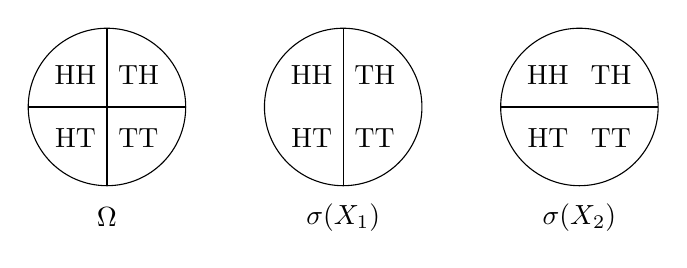
\begin{tikzpicture}
                    \foreach \x in {0,3,6}{
                        \draw[xshift=\x cm] (0,0) circle [radius=1cm];
                        \node[xshift=\x cm] at (0.4,0.4) {TH};
                        \node[xshift=\x cm] at (-0.4,0.4) {HH};
                        \node[xshift=\x cm] at (-0.4,-0.4) {HT};
                        \node[xshift=\x cm] at (0.4,-0.4) {TT};
                    }
                    \draw (1,0) -- (-1,0);
                    \draw (0,1) -- (0,-1);

                    \draw (3,1) -- (3,-1);

                    \draw (5,0) -- (7,0);

                    \node at (0,-1.4) {$\Omega$};
                    \node at (3,-1.4) {$\sigma(X_1)$};
                    \node at (6,-1.4) {$\sigma(X_2)$};
                \end{tikzpicture}
            \end{center}
            \begin{align*}
                \sigma(X_1)= \{\{H\} \times \{H, T\}, \{T\} \times \{H, T\}, \emptyset, \Omega\} \\
                \sigma(X_2)= \{\{H, T\} \times \{H\}, \{H, T\} \times \{T\}, \emptyset, \Omega\}
            \end{align*}
    \end{itemize}
\end{eg}

\begin{lemma}
    Let $\mathcal{F}_i \subseteq \mathcal{A}_i$ be a subfamily of events which is stable under finite intersection, such that $\sigma(\mathcal{F}_i) = \mathcal{A}_i$.
    Then to check that $(\mathcal{A}_i)_{i \geq 1}$ forms an independent family it is enough to check that
    \begin{equation*}
        \Prob\left(\bigcap_{i \in I} A_i\right) = \prod_{i \in I} \Prob(A_i)
    \end{equation*}
    holds $\forall I \subseteq \N$ finite and $\forall A_i \in \mathcal{F}_i$.
\end{lemma}

\begin{eg}\leavevmode
    \begin{enumerate}[label=(\alph*)]
        \item Let $(X_1, \dotsc, X_n)$ be \hyperlink{def:rv}{random variables}.
            They are \hyperlink{def:indepRV}{independent} $\iff$
            \begin{equation*}
                \forall x_1, \dotsc, x_n \in \mathbb{R} \quad \Prob(\forall i=1,\dotsc,n\; X_i \leq x_i) = \prod_{i=1}^n \Prob(X_i \leq x_i).
            \end{equation*}
            Indeed this is a special case of the lemma setting
            \begin{equation*}
                \mathcal{F}_i = \set{X_i^{-1}((-\infty, x]) | x \in \R} %)
            \end{equation*}
        \item If $X_1, \dotsc, X_n$ take only a finite set $E$ of values.
            $(X_1, \dotsc X_n)$ independent $\iff$
            \begin{equation*}
                \forall e_1, \dotsc, e_n \in E \quad \Prob(\forall i \; X_i = e_i) = \prod_{i=1}^n \Prob(X_i = e_i).
            \end{equation*}
    \end{enumerate}
\end{eg}

\begin{proof}[Proof of lemma]
    For two $\sigma$-subalgebras $\mathcal{A}_1$ and $\mathcal{A}_2$, let $A_2 \in \mathcal{A}_2$ be such that
    \begin{equation*}
        \Prob(A \cap A_2) = \Prob(A) \Prob(A_2) \tag{$*$} \label{eq:indepstar}
    \end{equation*}
    holds for all $A \in \mathcal{F}_1$.
    Look at the two measures
    \begin{align*}
        A &\longmapsto \Prob(A \cap A_2) \\
        A &\longmapsto \Prob(A) \Prob(A_2).
    \end{align*}
    The two measures coincide on $\mathcal{F}_1$, hence they coincide on $\mathcal{A}_1$ (by \hyperlink{lem:dynkin}{Dynkin's lemma}).
    So \eqref{eq:indepstar} holds $\forall A \in \mathcal{A}_1$.
    Now just reverse the roles of $\mathcal{A}_1$ and $\mathcal{A}_2$.
\end{proof}

\begin{eg}
    $\Omega = [0, 1]$, $\Prob =$ \hyperlink{def:lebMeas}{Lebesgue measure}, $\mathcal{F} = \mathcal{B}(\R)$ the \hyperlink{def:borelAlg}{Borel $\sigma$-algebra}.
    Let $X_n(\omega)$ be the $n$th digit of the decimal expansion of $\omega \in [0, 1]$.

    Claim $(X_n)_{n \geq 1}$ is \hyperlink{def:indepRV}{independent}. We have $X_n(\omega) \in \{0, 1, \dotsc, 9\}$.
    Let
    \begin{align*}
        I_{\epsilon_1, \dotsc, \epsilon_n} &= \set{\omega \in \Omega | X_1(\omega) = \epsilon_1, \dotsc, X_n(\omega) = \epsilon_n} \\
                                           &= \set{\omega \in [0, 1] | \floor{10^n \omega} = \epsilon_1 \dotsm \epsilon_n}.
    \end{align*}
    We need to check that
    \begin{align*}
        \Prob(X_1(\omega) = \epsilon_1, \dotsc, X_n(\omega) = \epsilon_n) &= \prod_{i=1}^n \Prob(X_i(\omega) = \epsilon_i) \\
                                                                          &= \prod_{i=1}^n \frac{1}{10} = \frac{1}{10^n}
    \end{align*}
    but it is clear $\Prob(\omega \in I_{\epsilon_1, \dotsc, \epsilon_n}) = \frac{1}{10^n}$.
\end{eg}

\begin{remark}\leavevmode
    \begin{itemize}
        \item If $f_1, \dotsc, f_n$ are \hyperlink{def:borelFunc}{Borel measurable functions} $\R \to \R$ and $X_1, \dotsc, X_n$ are \hyperlink{def:indepRV}{independent} \hyperlink{def:rv}{random variables}, then so are $f_1(X_1), \dotsc, f_n(X_n)$.
            So $\sigma(f(X)) \subseteq \sigma(X)$.
        \item \hyperlink{def:indepRV}{Independence} implies pairwise independence, but not conversely.
            Consider Bernstein's example: Take $X$,$Y$ two independent coin tosses.
            $X=1$ for heads, $X=0$ for tails, same for $Y$.
            Set $Z=\abs{X-Y}$, then we have pairwise independence but not independence.
    \end{itemize}
\end{remark}

\begin{prop}
    Let $X_1, \dotsc, X_n$ be $n$ \hyperlink{def:rv}{random variables}.
    \begin{equation*}
        (X_1, \dotsc, X_n) \text{ are \hyperlink{def:indepRV}{mutually independent}} \iff \mu_{(X_1, \dotsc, X_n)} = \mu_{X_1} \otimes \dotsb \otimes \mu_{X_n}.
    \end{equation*}
    \hypertarget{def:jointLaw}Here $\mu_{(X_1, \dotsc, X_n)}$ is the \hyperlink{def:law}{law or distribution} of $(X_1, \dotsc, X_n)$, and we say it's the joint law or joint distribution.
\end{prop}

\begin{proof}
    \begin{align*}
        \mu_{(X_1, \dotsc, X_n)} \left(\prod_{i=1}^n (-\infty, x_i]\right) &= \Prob\left((X_1, \dotsc, X_n) \in \prod_{i=1}^n (-\infty, x_i]\right) \\
                                                                &= \Prob(\forall i, X_i \leq x_i).
    \end{align*}
    \begin{align*}
        \text{independence } &\iff \forall x_i \in \R, \quad \Prob(\forall i, X_i \leq x) = \prod_{i=1}^n \Prob(X_i \leq x_i) \\
                             &\iff \mu_{(X_1, \dotsc, X_n)} \left(\prod_{i=1}^n (-\infty, x_i]\right) = \prod_{i=1}^n \mu_{x_i} ((-\infty, x_i]) \qedhere %)
    \end{align*}
\end{proof}

% lecture 14

\begin{prop}
    Suppose $X$ and $Y$ are two \hyperlink{def:indepRV}{independent} \hyperlink{def:rv}{random variables}.
    Assume $X$, $Y$ \hyperlink{def:integral}{integrable}, i.e.\ $\E(\abs{X}) < \infty,\ \E(\abs{Y}) < \infty$.
    Then $XY$ is integrable and
    \begin{equation*}\E(XY) = \E(X)\E(Y).\tag{$*$}\label{eq:indepExp}\end{equation*}
    Moreover \eqref{eq:indepExp} holds also if $X$ and $Y$ are just assumed $\geq 0$.
\end{prop}

\begin{proof}
    Recall that $X$, $Y$ are independent $\iff$ the \hyperlink{def:jointLaw}{joint law} $\mu_{(X,Y)}$ is the product $\mu_{(X,Y)} = \mu_X \otimes \mu_Y$ where $\mu_X=$ \hyperlink{def:law}{law} of $X$ and $\mu_Y=$ law of $Y$.
    So we can apply \hyperlink{thm:tonelliFubini}{Fubini}: $\E(X) = \int_\R x \, d \mu_X$, $\E(Y) = \int_\R y \, d \mu_Y$.
    \begin{equation*}
        \E(XY) = \int_{\R \times \R} xy \, d\mu_{(X,Y)}. \qedhere
    \end{equation*}
\end{proof}

\begin{lemma}[1st Borel-Cantelli lemma]\hypertarget{lem:bc1}
    Take $(\Omega, \mathcal{F}, \Prob)$ a \hyperlink{def:probabilitySpace}{probability space}.
    Let $(A_n)_{n \geq 1}$ be a sequence of events.
    Assume $\sum_{n \geq 1} \Prob(A_n) < \infty$.
    Then $\Prob(\lim \sup A_n) = 0$.
\end{lemma}
\begin{proof}
    \begin{align*}
        \limsup A_n &\coloneqq \bigcap_{m \geq 1} \bigcup_{n \geq m} A_n \\
        \Prob(\limsup A_n) &\leq \Prob\left(\bigcup_{n \geq m} A_n\right) \\
                             &\leq \sum_{n \geq m} \Prob(A_n) \to 0 \text{ as } m \to \infty.\qedhere
    \end{align*}
\end{proof}

\begin{eg}
    Take $\Omega = [0, 1]$. $\Prob=$ \hyperlink{def:lebMeas}{Lebesgue}, $\mathcal{F}=$ \hyperlink{def:borelAlg}{Borel $\sigma$-algebra}.
    A number $\alpha \in \R$ is said to be very-well-approximated if $\exists \epsilon > 0$ such that there are infinitely many integers $p,q$ such that
    \begin{equation*}
        \abs{\alpha - \frac{p}{q}} \leq \frac{1}{q^{2 + \epsilon}}.
    \end{equation*}
    Claim: Lebesgue \hyperlink{def:ae}{a.e.}\ numbers $\alpha$ are not very-well-approximated.
    Proof: (exercise) Apply \hyperlink{lem:bc1}{Borel-Cantelli} to the events
    \begin{equation*}
        A_q = \Set{x \in [0, 1] | d(q x, \Z) < \frac{1}{q^{1 + \epsilon}}}.
    \end{equation*}
\end{eg}

\begin{lemma}[2nd Borel-Cantelli lemma]\hypertarget{lem:bc2}
    Conversely to the \hyperlink{lem:bc1}{first Borel-Cantelli lemma}, assume that the events $(A_n)_{n \geq 1}$ are \hyperlink{def:independentEvents}{independent} and $\sum_{n \geq 1} \Prob(A_n) = + \infty$.
    Then $\Prob(\limsup A_n) = 1$.
\end{lemma}

\begin{remark}
    The conclusion fails without the assumption of independence, for instance take $A_n = [0, \frac{1}{n}] \subseteq \Omega = [0, 1]$, for which $\sum \Prob(A_n) = \sum \frac{1}{n} = \infty$, but $\lim \sup A_n = \{0\}$.
\end{remark}

\begin{proof}
    \begin{align*}
        \lim \sup A_n &= \bigcap_{m \geq 1} \bigcup_{n \geq m} A_m \\
        (\lim \sup A_n)^c &= \bigcup_{m \geq 1} \bigcap_{n \geq m} (A_m)^c \\
    \end{align*}
    but $\forall m$,
    \begin{align*}
        \Prob\left(\bigcup_{n \geq m} A_n^c\right)&= \prod_{n \geq m} \Prob(A_n^c) = \prod_{n \geq m} 1-\Prob(A_n) \\
                                                  &\leq \prod_{n \geq m} e^{-\Prob(A_n)} = e^{-\sum_{n \geq m} \Prob(A_n)} \\
                                                  &\to e^{-\infty} = 0.
    \end{align*}
\end{proof}

\begin{defi}[Random process]\hypertarget{def:randomProcess}
    A \textbf{random process} is an infinite family of $(X_n)_{n \geq 1}$ of real \hyperlink{def:rv}{random variables}, where $n$ can be thought of as a time parameter.
    We use $\mathcal{F}_n = \sigma(X_1, \dotsc, X_n) =$ the smallest sub-$\sigma$-algebra of $\mathcal{F}$ which makes all $X_i$, $i \leq n$ measurable.
    We also have $\mathcal{F}_{n+1} \supseteq \mathcal{F}_n$, the time filtration property.
\end{defi}

\begin{defi}[Tail $\sigma$-algebra]\hypertarget{def:tailAlg}
    The \textbf{tail $\sigma$-algebra} of $(X_n)_{n \geq 1}$ is defined as
    \begin{equation*}
        \tau = \bigcap_{n \geq 1} \sigma(X_n, X_{n+1}, \dotsc).
    \end{equation*}
\end{defi}

\begin{eg}
    The following events belong to \hyperlink{def:tailAlg}{$\tau$}:
    \begin{equation*}
        \{\lim \sup X_n \geq T\} \qquad \set{\omega \in \Omega | (X_n(\omega))_{n \geq 1} \text{ converges}}.
    \end{equation*}
\end{eg}

\begin{thm}[Kolmogorov 0-1 Law]\hypertarget{thm:kol01}
    Suppose $(X_n)_{n \geq 1}$ is a sequence of \hyperlink{def:indepRV}{independent} \hyperlink{def:rv}{random variables}.
    Then the \hyperlink{def:tailAlg}{tail $\sigma$-algebra} $\tau$ is trivial ($\forall A \in \tau, \Prob(A) \in \{0, 1\}$).
\end{thm}

\begin{proof}
    Let $A \in \tau$ and let $B \in \sigma(X_1, \dotsc, X_n)$.
    Then $A$ and $B$ are independent, because $\sigma(X_1, \dotsc, X_n)$ and $\tau$ are independent.
    So $\Prob(A \cap B) = \Prob(A) \cdot \Prob(B)$.

    Now the measures
    \begin{align*}
        B & \longmapsto \Prob(A \cap B) \\
        B & \longmapsto \Prob(A)\Prob(B)
    \end{align*}
    coincide on $\sigma(X_1, \dotsc, X_n)$ for all $n$, hence they coincide on $\sigma(X_1, \dotsc, X_n, \dotsc)$.
    But $\tau \subseteq \sigma(X_1, \dotsc, X_n, \dotsc)$.
    In particular $\Prob(A \cap A) = \Prob(A) \cdot \Prob(A)$ so $\Prob(A)=\Prob(A)^2$ hence $\Prob(A) = \{0,1\}$.
\end{proof}

\begin{eg}\leavevmode
    \begin{itemize}
        \item Take an i.i.d.\ space $(X_n)_{n \geq 1}$ of \hyperlink{def:rv}{random variables} such that $\forall T \geq 0$, $\Prob(X_1 < T) < 1$.
            Then almost surely $\lim \sup X_n = +\infty$.

            Indeed,
            \begin{equation*}
                \sum_{k=1}^n \Prob(X_n \geq T) = n \Prob(X_1 \geq T) = n(1 - \Prob(X_1 < T)) \to \infty
            \end{equation*}
            so the \hyperlink{lem:bc2}{second Borel-Cantelli lemma} applies and $\Prob(\limsup A_n) = 1$.
        \item Take $(\epsilon_n)_{n \geq 1}$ be i.i.d.\ random variables with $\Prob(\epsilon_1 = 1) = \Prob(\epsilon_1 = -1) \frac{1}{2}$.
            Take $(a_n)_{n \geq 1}$ some sequence of real numbers, and ask when does $\sum_{n \geq 1} \epsilon_n a_n$ converge?

            The \hyperlink{thm:kol01}{Kolmogorov 0-1 law} tells us that this happens with probability $0$ or $1$ depending only on the sequence $(a_n)_{n \geq 1}$.
            In fact, a theorem of Rademacher-Paley-Zygmund says
            \begin{equation*}
                \sum_{n=1}^\infty \epsilon_n a_n \text{converges a.s.} \iff \sum_{n=1}^\infty a_n^2 < \infty.
            \end{equation*}
    \end{itemize}
\end{eg}

Take $\mu$ a \hyperlink{def:probMeas}{probability measure} on $\mathbb{R}$.
Can you find a \hyperlink{def:probabilitySpace}{probability space} $(\Omega, \mathcal{F}, \Prob)$ and a \hyperlink{def:rv}{random variable} $X$ such that $\mu$ is the law of $X$?

Yes: Take $\Omega = \R$, let $\mathcal{F}$ be the Borel sets, and set $\Prob = \mu$, and $X(\omega) = \omega$.

\begin{defi}[Moment]\hypertarget{def:moment}
    If $X$ is a \hyperlink{def:rv}{random variable}, the \textbf{$k$th moment} of $X$ is $\E(X^k)$ for $k \in \N$.
\end{defi}
% 8 nov

Some additional basic terminology:
\hypertarget{def:mean}For $X$ a \hyperlink{def:rv}{random variable}, $\mathbb{E}(X)$ is called the mean, and $\mathbb{E}((X - \mathbb{E}X)^2)$ is the variance of $X$, denoted $\Var X$.

\begin{remark}\leavevmode
    \begin{itemize}
        \item $\Var(X) = \mathbb{E}(X^2) - (\mathbb{E}X)^2$
        \item If $X, Y$ are independent then $\Var(X + Y) = \Var(X) + \Var(Y)$.
    \end{itemize}
\end{remark}

\begin{thm}[Strong law of large numbers (under a \hyperlink{def:moment}{4th moment} assumption)]\hypertarget{thm:sll}
    Let $(X_n)_{n \geq 1}$ be a sequence of \hyperlink{def:indepRV}{independent} and identically distributed (i.i.d.)\ \hyperlink{def:rv}{random variables} with common \hyperlink{def:law}{law} $\mu$.
    Assume $\int_\R x^4 \, d\mu(x) < \infty$ (i.e.\ $\mathbb{E}(\abs{X_1}^4) < \infty$).
    Then
    \begin{equation*}
        \frac{1}{n} \sum_{k=1}^n X_k \xrightarrow{n \to \infty} \mathbb{E}(X_1)
    \end{equation*}
    almost surely.
\end{thm}

\begin{eg}
    Take $\Omega = [0, 1]$ and $\mathbb{P} = $ Lebesgue.
    Write $\omega = 0.\epsilon_1 \epsilon_2 \dotsc \epsilon_n \dotsc$ with $\epsilon_i \in \{0, \dotsc, 9\}$, the decimal expansion of $\omega$.
    We observed that $(\epsilon_n(\omega))_{n \geq 1}$ were \hyperlink{def:indepRV}{independent} and uniformly distributed in $\{0, \dotsc, 9\}$.
    Set $X_n^{(i)} (\omega) = \1{\epsilon_n(\omega) = i}$, these are i.i.d.\ \hyperlink{def:rv}{random variables} and $\abs{X_n^{(i)}} \leq 1$, so finite fourth moment.
    So the \hyperlink{thm:sll}{SLL} applies:
    \begin{equation*}
        \frac{1}{n} \sum_{k=1}^n X_k^{(i)} = \frac{1}{n} \# \{k \leq n, \epsilon_k(\omega) = i\} \implies \mathbb{E}(X_1^{(k)}) = \frac{1}{10}.
    \end{equation*}
    So, for Lebesgue \hyperlink{def:ae}{almost every} $\omega$ the proportion of each digit is the same (a normal number).
\end{eg}
\begin{thm}[Borel]
    \hyperlink{def:ae}{Almost every} number is a normal number.
\end{thm}

\begin{lemma}[Cauchy-Schwarz inequality]
    Take $f, g$ square integrable functions on $(X, \mathcal{A}, \mu)$ then $fg$ is integrable and
    \begin{equation*}
        \abs{\int fg \, d\mu} \leq \sqrt{\int f^2 \, d\mu} \sqrt{\int g^2 \, d \mu}.
    \end{equation*}
    Equivalently, take $X$, $Y$ random variables such that $\mathbb{E}(X^2) < \infty$ and $\mathbb{E}(Y^2) < \infty$, then $\mathbb{E}(\abs{XY}) \leq \sqrt{\mathbb{E}X^2 \mathbb{E}Y^2}$.
\end{lemma}

\begin{proof}
    Look at $t \mapsto \mathbb{E}((X + t Y)^2) = \mathbb{E}X^2 + t^2 \mathbb{E} Y^2 + 2 t \mathbb{E}(XY) \geq 0$ $\forall t \in \R$.
    So, $\Delta = 4 (\mathbb{E}(XY))^2 - 4 \mathbb{E}X^2 \mathbb{E}Y^2 \leq 0$.
\end{proof}

\begin{proof}[Proof of the strong law of large numbers]
    Without loss of generality, assume that $\mathbb{E}(X_1) = 0$, because we can replace $X_n$ by $X_n - \mathbb{E}(X_1)$.
    This is allowed because $\mathbb{E}((X_n - \mathbb{E}X_1)^4) < \infty$.
    Indeed,
    \begin{align*}
        (X_n - \mathbb{E}X_1)^4 &= [(X_n - \mathbb{E}X_1)^2]^2 \\
                                &\leq (2X_n^2 + 2(\mathbb{E}X_1)^2)^2 \\
                                &\leq 8 [X_n^4 + (\mathbb{E}X_1)^4].
    \end{align*}
    So we have $\mathbb{E}(X_n) = 0$ $\forall n$.

    Let $S_n = \frac{1}{n} (X_1 + \dotsb + X_n)$, so $S_n^4  = \frac{1}{n^4} (\sum_{i,j,k,l} X_i X_j X_k X_l)$.
    By independence, $\mathbb{E}(X_i X_j X_k X_l) = 0$ if
    \begin{itemize}[label=--]
        \item $i, j, k, l$ are distinct, or
        \item $k = l$ and $i \neq j \notin \{k, l\}$ or
        \item $k = l = j \neq i$.
    \end{itemize}
    So,
    \begin{align*}
        \mathbb{E}(S_n^4) &= \frac{1}{n^4} \left(\mathbb{E}X_1^4 + \dotsb + \mathbb{E}X_n^4 + 6 \sum_{i < j} \mathbb{E}X_i^2 \cdot \mathbb{E}X_j^2\right) \\
                          &= \frac{1}{n^4} \left(n \mathbb{E}X_i^4 + 6 \frac{n(n-1)}{2} \left(\mathbb{E}(X_1^2)\right)^2\right) \\
                          &= \mathcal{O}\left(\frac{1}{n^2}\right).
    \end{align*}
    So in conclusion,
    \begin{equation*}
        \begin{aligned}
            \sum_{n \geq 1} \E(S_n^4) = \E\left(\sum_{n \geq 1} S_n^4\right) < \infty
        \end{aligned}
    \end{equation*}
    So $\sum_{n \geq 1} S_n^4 < \infty$ a.s. $\implies \lim_{n\to \infty} S_n = 0$ almost surely.
\end{proof}

\clearpage
\section{Type of convergence of random variables}
\begin{notation}\hypertarget{def:cb}
    $C_b(\R^d)$ is the space of continuous and bounded real functionals on $\R^d$.
\end{notation}

\begin{defi}[Weak convergence]\hypertarget{def:weakConv}
    A sequence of \hyperlink{def:probMeas}{probability measures} on $(\R^d, \mathcal{B}(\R^d))$, say $(\mu_n)_{n \geq 1}$ is said to \textbf{converge weakly} to a measure $\mu$ on $(\R^d, \mathcal{B}(R^d))$ if
    \begin{equation*}
        \forall f \in \hyperlink{def:cb}{C_b(\R^d)} \quad \mu_n(f) \xrightarrow{n \to \infty} \mu(f).
    \end{equation*}
\end{defi}
\begin{eg}
    \leavevmode
    \begin{itemize}
        \item $\mu_n = \delta_{x_n}$ a Dirac mass,
            \begin{equation*}
                \delta_x(A) =
                \begin{cases}
                    1 & x \in A \\
                    0 & x \notin A
                \end{cases}
                \quad \text{for } x \in \R^d
            \end{equation*}
            with $x_n \in \R^d$ with $x_n \to x \in \R^d$ then clearly $\mu_n \to \delta_x$ weakly.
        \item $\mu_n = \mathcal{N}(0, \sigma_x^2)$, the centered Gaussian with standard deviation $\sigma_x$. If $\sigma_x \to 0$ then $\mu_n \to \delta_0$ weakly.
    \end{itemize}
\end{eg}

\begin{defi}[Convergence]\hypertarget{def:conv}
    A sequence of $\R^d$-valued \hyperlink{def:rv}{random variables} $(X_n)_{n \geq 1}$ is said to converge to $X$
    \begin{enumerate}[label=(\alph*)]
        \item \textbf{almost surely} if for $\mathbb{P}$ a.e.\ $\omega$, $X_n(\omega) \xrightarrow{n \to \infty} X(\omega)$
        \item \textbf{in probability} (or in measure) if $\forall \epsilon > 0$, $\mathbb{P}(\norm{X_n - X} > \epsilon) \xrightarrow{n \to \infty} 0$.
        \item \textbf{in distribution} if $\mu_{X_n} \xrightarrow{n \to \infty} \mu_X$ weakly, with $\mu_{X_n}$ the \hyperlink{def:law}{law} of $X_n$ on $\mathbb{R}^d$.
    \end{enumerate}
\end{defi}

\begin{remark}
    (a) $\Rightarrow$ (b) $\Rightarrow$ (c), but none of the reverse implications hold in general.

    (a) $\Rightarrow$ (b): $\Prob(\|X_n-X\| > \epsilon) = \mathbb{E}(\1{\|X_n-X\| > \epsilon}) \xrightarrow{n \to \infty} 0$ by \hyperlink{thm:dct}{Lebesgue Dominated Convergence}.

    (b) $\Rightarrow$ (c): Let $f \in \hyperlink{def:cb}{C_b(\R^d)}$. $f$ is uniformly continuous on compact subsets of $\R^d$.
    So $\forall \epsilon>0$, $\exists \delta >0$ such that if $\|x\| < 1/\epsilon$ and $\|x-y\| < \delta$, then $|f(x) - f(y)| < \epsilon$. So
    \begin{align*}
        |\mu_n (f) - \mu(f)| &\leq \E(|f(X_n) - f(X)|)\\
                             &
        \begin{multlined}
            \leq\E\left(\1{\|X_n-X\|<\delta}\1{\|X\|<\frac{1}{\epsilon}} |f(X_n) -f(X)|\right) \\
            \hspace{10em} +2\|f\|_\infty \Prob\left(\|X_n-X\|>\delta \text{ or } \|X\|>\frac{1}{\epsilon}\right)
        \end{multlined}
        \\
        &\leq \epsilon+2\|f\|_\infty [\Prob(\|X_n-X\|>\delta ) + \Prob(\|X\|>1/\epsilon)]
    \end{align*}
    So
    \begin{align*}
        \limsup_n |\mu_n(f) - \mu(f)| \leq \epsilon+2\|f\|_\infty \Prob(\|X\|>1/\epsilon) \xrightarrow{\epsilon \to 0} 0.
    \end{align*}

    When $d=1$, (c) is equivalent to saying that the \hyperlink{def:cdf}{distribution function} $F_{\mu_n} (X) \to F_\mu(x)$ for all $x \in \R$ where $F_\mu(x)$ is continuous.
    Recall
    \begin{align*}
        F_\mu(x) &\coloneqq \mu((-\infty,x]) \\ %)
        F_{\mu_n}(x) &\coloneqq \mu_n((-\infty,x]). %)
    \end{align*}
    For example, take $\mu_n = \delta_{1/n} \to \delta_0 = \mu$, so $F_{\mu_n} = \1{x \geq \frac{1}{n}}$, but $F_\mu = \1{x \geq 0}$.
    Then $F_{\mu_n}(0) = 0$ while $F_\mu(0) = 1$, so $F_{\mu_n}(0) \not\to F_\mu(0)$.
\end{remark}

\begin{prop}
    If $(X_n)_{n \geq 1}$ \hyperlink{def:conv}{converges in probability} to $X$, then $\exists$ a subsequence $(X_{n_k})_{k \geq 1}$ such that $X_{n_k} \xrightarrow{k \to \infty} X$ \hyperlink{def:conv}{almost surely}.
\end{prop}
\begin{proof}
    For all $k$ we have
    \begin{gather*}
        \Prob\left(\|X_n - X\| > \frac{1}{k}\right) \xrightarrow{n \to \infty} 0\\
        \implies \exists n_k \text{ such that } \mathbb{P}\left(\|X_{n_k}-X\| > \frac{1}{k}\right) \leq \frac{1}{2^k}.
    \end{gather*}
    So
    \begin{equation*}
        \sum \mathbb{P}\left(\|X_{n_k}-X\| > \frac{1}{k}\right) < \infty \implies \mathbb{P}\left(\limsup \|X_{n_k} - X\| > \frac{1}{k}\right) = 0.
    \end{equation*}
    by \hyperlink{lem:bc1}{Borel-Cantelli}.
\end{proof}

\begin{defi}[$L^1$ convergence]\hypertarget{def:l1}
    A sequence of $\mathbb{R}^d$-valued \hyperlink{def:integral}{integrable} \hyperlink{def:rv}{random variables} $(X_n)_{n \geq 1}$ \textbf{converges in $L^1$} (or in mean)
    towards an integrable random variable $X$ if
    \begin{align*}
            \E(\|X_n-X\|) \xrightarrow{n \to \infty} 0
    \end{align*}
    which we'll write $X_n \xrightarrow{L^1} X$.
\end{defi}

\begin{remark}\leavevmode
    \begin{itemize}
        \item if $X_n \hyperlink{def:l1}{\xrightarrow{L^1}} X$ then $X_n \to X$ in \hyperlink{def:conv}{probability}. Indeed, $\forall \epsilon>0$,
            \begin{equation*}
                    \epsilon \Prob(\|X_n-X\| > \epsilon) \leq \E(\|X_n - X\| \1{\|X_n-X\|>\varepsilon}) \leq \E(\|X_n-X\|).
            \end{equation*}
        \item This demonstrates the Markov inequality,
            \begin{equation*}
                    \epsilon\Prob(|X| \geq \epsilon) \leq \E(|X|)
            \end{equation*}
            holds for any \hyperlink{def:rv}{random variable} $X$ and any $\epsilon > 0$.
        \item The Markov inequality gives also the Chebyshev inequality,
            \begin{equation*}
                    \epsilon^2 \Prob(|X-\E X| > \epsilon) \leq \Var X
            \end{equation*}
            holds for any \hyperlink{def:rv}{random variable} $X$ and any $\epsilon > 0$.
    \end{itemize}
\end{remark}

In general, the converse does not hold, i.e.\ convergence in probability $\not \Rightarrow$ in $L^1$.
\begin{eg}
    For example, take $\Omega = [0,1]$, $\Prob =$ Lebesgue and $X_n = n \1{[0,\frac 1n]}$.
    Then $X_n \to 0$ \hyperlink{def:conv}{in probability} (since $\Prob(|X_n| > \epsilon) = \frac{1}{n}$) but $\mathbb{E}(X_n) = 1$ for any $n$.
\end{eg}

If $\exists M \geq 0$ such that $\|X_n\| \leq M$ almost surely for all $n$, then the converse holds.
\begin{align*}
    \E(\|X_n - X\|) &= \E(\|X_n - X\|\1{\|X_n-X\| \leq \epsilon}) + \E(\|X_n - X\|\1{\|X_n-X\| > \epsilon}) \\
    &\leq \epsilon + 2 M \Prob(\|X_n - X\| > \epsilon).
\end{align*}
so $\limsup \E(\|X_n - X\|) \leq \epsilon$.

\begin{defi}[Uniform integrability]\hypertarget{def:ui}
    A sequence of \hyperlink{def:integral}{integrable} \hyperlink{def:rv}{random variables} $(X_n)_{n \geq 1}$ is called \textbf{uniformly integrable} if
    \begin{equation*}
            \sup_{n \geq 1} \E(\|X_n\| \1{\|X_n\|>M}) \xrightarrow{M \to \infty} 0.
    \end{equation*}
\end{defi}

\begin{remark}\leavevmode
    \begin{itemize}
        \item If $X_n = X$ for all $n$, and $X$ is \hyperlink{def:integral}{integrable}, then $(X_n)_n$ is \hyperlink{def:ui}{uniformly integrable}:
            \begin{equation*}
                \E(\|X\|\1{\|X\|\leq M}) \uparrow \E(\|X\|)
            \end{equation*}
            as $M \to \infty$ by \hyperlink{def:monConv}{monotone convergence}, so
            \begin{equation*}
                \E(\|X\| \1{\|X\|> M}) \xrightarrow{M \to \infty} 0.
            \end{equation*}

        \item Suppose the $X_n$s are dominated, i.e.\ there is some $Y$ an integrable \hyperlink{def:rv}{random variable} such that $\|X_n\|\leq Y$ for all $n$. Then $(X_n)_n$ are \hyperlink{def:ui}{uniformly integrable}:
            \begin{equation*}
                \E(\|X_n\| \1{\|X_n\| > M}) \leq \E(Y \1{Y>M}) \xrightarrow{M \to \infty} 0.
            \end{equation*}

        \item If $X_n \hyperlink{def:l1}{\xrightarrow{L^1}} X$, then $(X_n)_n$ is \hyperlink{def:ui}{uniformly integrable}:
            \begin{align*}
                    \E(\|X_n\|\1{\|X_n\|>M}) &\leq \E(\|X_n-X\| \1{\|X_n\|>M}) + \E(\|X\| \1{\|X_n\|>M})\\
                                             &\leq
                    \begin{aligned}[t]
                        \E(\|X_n-X\|) &+ \E(\|X\|\1{\|X\|>M} \1{\|X_n\|>M}) \\
                                      &+ \E(\|X\| \1{\|X\| < M} \1{\|X_n\|>M})
                    \end{aligned}
                    \\
                                             &\leq \E(\|X_n-X\|) + \E(\|X\| \1{\|X\|>M}) + M\E(\1{\|X_n\| \geq M}) \\
                                             &\leq \E(\|X_n-X\|) + \epsilon M.
            \end{align*}
            % So $M \Prob(\|X_n\| > M) \leq \E(\|X_n\|) \to \E(\|X\|)$.
    \end{itemize}
\end{remark}
\begin{thm}
    Let $(X_n)_{n \geq 1}$ be a sequence of \hyperlink{def:integral}{integrable} \hyperlink{def:rv}{random variables}, and let $Y$ be another random variable.
    Then $(X_n)$ is \hyperlink{def:ui}{uniformly integrable} and \hyperlink{def:conv}{converges in probability} to $X$ if and only if $X$ is integrable and $X_n \hyperlink{def:l1}{\xrightarrow{L^1}} X$.
\end{thm}
\begin{proof}[Proof of $(\Rightarrow$).]
    Suppose $(X_n)$ is \hyperlink{def:ui}{uniformly integrable} and \hyperlink{def:conv}{converges to $X$ in probability}.
    We've shown that there is a subsequence $(X_{n_k})_k$ such that $X_{n_k} \xrightarrow{k \to \infty} X$ almost surely.
    \begin{equation*}
        \E(\|X\| \1{\|X\| \geq M}) \leq \liminf_{n \to \infty} \E(\|X_{n_k}\| \1{\|X_{n_k}\| > M}) = \epsilon M
    \end{equation*}
    by \hyperlink{thm:fatou}{Fatou's lemma}.

    So $\E(\|X\|) = \E(\|X\|\1{\|X\| < M}) + \E(\|X\|\1{\|X\| \geq M}) \leq M + \epsilon M < \infty$ so $X$ is integrable.
    Hence \textbf{rest of the proof missing}.
\end{proof}
\begin{remark}
    This theorem subsumes the \hyperlink{thm:dct}{Lebesgue Dominated Convergence theorem}.
    If $\exists C > 0$ and some $p>1$ such that $\E(\|X_n\|^p) \leq C$ for any $n$ then $(X_n)_n$ is \hyperlink{def:ui}{uniformly integrable}.
    Indeed
    \begin{align*}
        M^{p-1} \E(\|X_n\| \1{\|X_n\| > M}) \leq \E(\|X_n\|^p) \leq C \\
        \shortintertext{so}
        \sup_n\E(\|X_n\| \1{\|X_n\| > M}) \leq \frac{C}{M^{p-1}} \xrightarrow{M \to \infty} 0.
    \end{align*}
\end{remark}
\textbf{missing end of section}
%For the $(\Leftarrow)$, need to show if $X_n \hyperlink{def:l1}{\xrightarrow{L^1}} X$ then $(X_n)_n$ is \hyperlink{def:ui}{uniformly integrable}.
%Observe that $(X_n)_n$ is uniformly integrable if and only if
%\begin{equation*}
%    \limsup_{n \to \infty} \E(\|X_n\|\1{\|X_n\|>M}) \xrightarrow{M \to \infty} 0.
%\end{equation*}
%This is because for any finitely many $X_1, \dotsc, X_{n_0}$,

\clearpage
\section{\texorpdfstring{$L^p$}{Lp} spaces}
\begin{prop}[H\"older inequality]\hypertarget{prop:holder}
    Let $p,q \in [1,\infty]$ such that $\frac 1p + \frac 1q = 1$ (taking $\frac 1\infty \coloneqq 0$).
    Let $f,g$ be \hyperlink{def:measurableFunc}{measurable functions} on a \hyperlink{def:measureSpace}{measure space} $(X, \mathcal{A},\mu)$. Then
    \begin{equation*}
        \int_X |fg| \, d\mu \leq \sqrt[p]{\int_X |f|^p \, d\mu}\sqrt[q]{\int_X |g|^q \, d\mu}
    \end{equation*}
    with equality iff $\exists a,b \in \mathbb{R}$ not both $0$ such that $a |f|^p = b |g|^q$ \hyperlink{def:ae}{$\mu$-almost everywhere}.
\end{prop}
\begin{proof}
    Without loss of generality, assume $p,q \in (1,\infty)$ and $\int |f|^p \, d\mu = 1 = \int |g|^q \, d\mu$ (up to changing $f,g$ by a scalar).
    The Young inequality for products gives
    \begin{equation*}
        \forall a,b \geq 0 \quad ab \leq \frac{1}{p} a^p + \frac{1}{q} b^q
    \end{equation*}
    (follows from convexity of $x \mapsto -\log x$, since
    \begin{equation*}
        \log(ta^p + (1-t) b^q) \geq t \log a^p + (1-t) \log b^q
    \end{equation*}
    and take $t = \frac{1}{p}$.)
    Write $|f(x) g(x)| \leq \frac{1}{p} |f(x)|^p + \frac{1}{q} |g(x)|^q$ and integrate, giving
    \begin{equation*}
        \int |fg| \, d\mu \leq 1. \qedhere
    \end{equation*}
\end{proof}

\begin{prop}[Minkowski inequality]\hypertarget{prop:mink}
    Take $p \in [1, \infty]$ and $f,g$ \hyperlink{def:measurableFunc}{measurable} functions on a \hyperlink{def:measureSpace}{measure space} $(X, \mathcal{A},\mu)$. Then
    \begin{equation*}
        \sqrt[p]{\int|f+g|^p \, d\mu} \leq \sqrt[p]{\int|f|^p \, d\mu}+\sqrt[p]{\int|g|^p \, d\mu}.
    \end{equation*}
\end{prop}
\begin{proof}
    For $p=1$, this follows by linearity of $\int$ so take $p > 1$. Apply \hyperlink{prop:holder}{H\"older} to $|f||f+g|^{p-1}$ and $|g||f+g|^{p-1}$:
    \begin{equation*}
        \int |f+g|^p \leq \int (|f|+|g|) |f+g|^{p-1} \leq \left(\sqrt[p]{\int|f|^p}+\sqrt[p]{\int|g|^p}\right) \sqrt[q]{\int|f+g|^{q(p-1)}}
    \end{equation*}
    and $q(p-1) = p$.
\end{proof}

\begin{remark}
    We need to check $\int |f+g|^p < \infty$ for this proof to make sense. But this follows from
    \begin{equation*}
        |f+g|^p \leq (2 \max\{|f|,|g|\})^p = 2^p \max \{|f|^p,|g|^p\} \leq 2^p (|f|^p + |g|^p)
    \end{equation*}
    so the integrability of $|f|^p$ and $|g|^p \implies \int |f+g|^p \, d\mu < \infty$.
\end{remark}
\begin{notation}
    \hypertarget{def:lpspacewrong}Write
    \begin{equation*}
        \mathcal{L}^p(X, \mathcal{A},\mu) = \left\{\mathcal{A}\text{-measurable functions $f$ on $X$ such that }\int_X |f|^p \, d\mu < \infty\right\}.
    \end{equation*}
\end{notation}
By the previous remark this is a real vector space.
\begin{defi}\hypertarget{def:lpnorm}
    The $L^p$-norm of $f$ is defined by $\|f\|_p =\sqrt[p]{\int|f|^p \, d\mu}$ for $1 \leq p < \infty$.
\end{defi}
The following hold:
\begin{itemize}
    \item $\|\alpha f \|_p = |\alpha| \|f\|_p$ for all $\alpha \in \mathbb{R}$
    \item $\|f+g\|_p \leq \|f\|_p + \|g\|_p$ (from \hyperlink{prop:mink}{Minkowski})
\end{itemize}
\begin{remark}
    If $\|f\|_p = 0$ then $f=0$ \hyperlink{def:ae}{$\mu$-a.e.}, so $\|\cdot\|_p$ is only a pseudo-norm on $\mathcal{L}^p(X, \mathcal{A},\mu)$.
    Note
    \begin{equation*}
        \text{if} \quad
        \begin{aligned}
            f_1 &= f_2\ \mu\text{-a.e.}\\
            g_1 &= g_2\ \mu\text{-a.e.}
        \end{aligned}
        \quad \text{then} \quad
        \begin{aligned}
            f_1+g_1 &= f_2+g_2\ \mu\text{-a.e.}\\
            f_1 g_1 &= f_2 g_2\ \mu\text{-a.e.}
        \end{aligned}
    \end{equation*}
    so if we say that two functions $f,g$ on $(X,\mathcal{A},\mu)$ are equivalent $f \sim_\mu g$ if $f-g = 0$ $\mu$-a.e. then this is an equivalence relation compatible with $+,\times$.
\end{remark}

\begin{defi}[$L^p$ space]\hypertarget{def:lpspace}
    Let $L^p(X, \mathcal{A},\mu)$ be the set of equivalence classes of functions in $\hyperlink{def:lpspacewrong}{\mathcal{L}^p(X,\mathcal{A},\mu)}$.
    Define $\|[f]\|_p = \|f\|_p$. This is a real vector space and $\|[f]\|_p$ is a genuine norm of $f$.

    When $p=\infty$ and $f$ a measurable function,
    \begin{equation*}
        \|f\|_\infty \coloneqq \inf \set{t \geq 0 | |f(x)| \leq t \text{ for } \mu\text{-a.e.} x}.
    \end{equation*}
\end{defi}
\begin{prop}[Completeness of \hyperlink{def:lpspace}{$L^p$ spaces}]
    \hyperlink{def:lpspace}{$L^p(X, \mathcal{A},\mu)$} for $p \in [1,\infty]$ is complete, i.e.\ every Cauchy sequence converges.
\end{prop}
\begin{proof}
    Let $(f_n)_{n \geq 1}$, $f_n \in \hyperlink{def:lpspacewrong}{\mathcal{L}^p(X, \mathcal{A},\mu)}$ and $\forall \epsilon\ \exists N$ with $\|f_n - f_m\|_p < \epsilon$ for all $n,m > N$.
    Pick a subsequence $n_k$ such that $f_{n_{k+1}} - f_{n_k} \leq \frac{\epsilon}{2^k}$ so $\sum_{k \geq 1} \|f_{n_{k+1}}-f_{n_k}\| \leq \epsilon$.
    By \hyperlink{prop:mink}{Minkowski},
    \begin{equation*}
        \left\|\sum_{k=1}^K \left|f_{n_{k+1}} - f_{n_k}\right| \right\|_p \leq \epsilon \quad \forall k < \infty.
    \end{equation*}
    Let $K \to \infty$ so by \hyperlink{def:monConv}{monotone convergence theorem} it holds also for $K = \infty$.
    Thus \hyperlink{def:ae}{$\mu$-a.e.}
    \begin{equation*}
        \sum_{k=1}^\infty \left|f_{n_{k+1}} - f_{n_k}\right|(x) < \infty
    \end{equation*}
    so for \hyperlink{def:ae}{$\mu$-a.e.\ }$x$, $(f_{n_k}(x))_k$ converges (by completeness of $\mathbb{R}$), let $f(x)$ be the limit.
    Outside this set of $x$s, just set $f(x) = 0$.

    Finally,
    \begin{equation*}
        \|f_n-f\|_p = \left\|\lim_{k \to \infty} (f_n - f_{n_k})\right\|_p \leq \liminf_{k \to \infty} \|f_n - f_{n_k}\|
    \end{equation*}
    by \hyperlink{thm:fatou}{Fatou's lemma} but since $f_n$ is Cauchy this is $\leq \epsilon$ if $n$ is large enough.
\end{proof}
So, \hyperlink{def:lpspace}{$L^p$ space} is a Banach space.
\begin{remark}[Approximation by simple functions]
    The vector space of \hyperlink{def:simpleFunc}{simple functions} of the form
    \begin{equation*}
        \sum_{i=1}^N a_i \1{A_i} \quad \text{where } a_i \in \mathbb{R}, A_i \in \mathcal{A} \text{ such that } \mu(A_i) < \infty
    \end{equation*}
    is dense in $L^p(X,\mathcal{A},\mu)$ for all $p \in [1,\infty]$.
    Namely if $f \in L^p(X,\mathcal{A},\mu)$ then let $f = f^+ - f^-$ and
    \begin{equation*}
        f_n^+ = \frac{2^n f^+}{2^n} \wedge n.
    \end{equation*}
    So $f_n^+$ a simple function. Similarly define $f_n^-$.
    Then $f_n^+ \to f^+$ and $f_n^- \to f^-$ \hyperlink{def:ae}{a.e.} and $|f_n| < 2|f|$.
    So when $p < \infty$ by \hyperlink{thm:dct}{dominated convergence} we get $\|f_n-f\|_p \xrightarrow{n \to \infty} 0$.
    When $p=\infty$ $\|f-f_n\|\leq \frac{1}{2^n}$.

    In particular $L^\infty \cap L^p$ is dense in $L^p$, since the simple functions are contained in $L^\infty \cap L^p$.
\end{remark}
\begin{remark}
    Take $X=\mathbb{R}^d$, $\mathcal{A}$ the \hyperlink{def:borelAlg}{Borel $\sigma$-algebra} and $\mu$=\hyperlink{def:lebMeas}{Lebesgue}.
    Then $C_c(\mathbb{R}^d)$ and $C_c^\infty (\mathbb{R}^d)$ are dense in $\hyperlink{def:lpspace}{L^p(\mathbb{R}^d, \mathcal{A},\mu)}$ when $p \in [1, \infty)$.
    Recall $C_c(\mathbb{R}^d)$ is the set of continuous functions with compact support and $C_c^\infty(\mathbb{R}^d)$ are the smooth functions with compact support.

    This fails for $p=\infty$, take for instance $f = \1{[0,1]}$
    \begin{center}
        \begin{tikzpicture}
            \draw (-0.5,0) -- (0,0) -- (0,1) -- (1,1) -- (1,0) -- (2.6,0);
            \node at (0,-0.2) {$0$};
            \node at (1,-0.2) {$1$};
        \end{tikzpicture}
    \end{center}
    then for any continuous $f$, $\|\1{[0,1]}-f\|_\infty \geq \frac 12$.
    % missing content

\end{remark}
\subsection{Hilbert spaces}
\begin{defi}[Hilbert space]\hypertarget{def:hilbert}
    A vector space $\mathcal{H}$ over $\mathbb{R}$ or $\mathbb{C}$ is called a \textbf{Hilbert space} if it is endowed with an inner product
    \begin{align*}
        \mathcal{H} \times \mathcal{H} &\longrightarrow \mathbb{R} \text{ or } \mathbb{C} \\
        (x,y) &\longmapsto \langle x,y\rangle
    \end{align*}
    such that
    \begin{itemize}
        \item $\langle x,x\rangle \in \mathbb{R}_+$ and $\langle x,x\rangle = 0 \implies x=0$
        \item $\overline{\langle x,y\rangle} = \langle y,x \rangle$ for any $x,y \in \mathcal{H}$
        \item $\langle x + \lambda x',y \rangle = \langle x+ y \rangle + \lambda \langle x',y\rangle$ $\forall \lambda \in \mathbb{R}$ or $\mathbb{C}$
    \end{itemize}
    and $\mathcal{H}$ is complete with respect to the norm $\|x\|\coloneqq \sqrt{\langle x,y\rangle}$.
\end{defi}

\begin{eg}
    \begin{itemize}
        \item $\mathcal{H}=\mathbb{R}^d$ with $\langle x,y\rangle = \sum_{i=1}^d x_i y_i$
        \item $\mathcal{H}=\mathbb{C}^d$ with $\langle x,y\rangle = \sum_{i=1}^d x_i \overline{y_i}$
        \item $\mathcal{H}=\hyperlink{def:lpspace}{L^2(X,\mathcal{A},\mu)}$ with $\langle f,g\rangle = \int_X fg \, d\mu$ as an $\mathbb{R}$ vector space.
    \end{itemize}
\end{eg}
\begin{lemma}[Existence of orthogonal projection]
    Let $\mathcal{H}$ be a \hyperlink{def:hilbert}{Hilbert space} and let $V$ be a closed vector subspace.
    Then $\forall x \in \mathcal{H}$, $\exists! y \in V$ such that $d(x,V) = \|x-y\|$ (where $d(x,V) \coloneqq \inf\set{\|x-z\| | z \in V}$).
\end{lemma}
\begin{proof}
    Pick a sequence $y_n \in V$ such that $\|x-y_n\| \to d(x,V)$. Then
    \begin{equation*}
        \left\|x-\frac{y_n+y_m}{2}\right\|^2
    \end{equation*}
\end{proof}

% missing a crapload

\clearpage
\begin{cor}
    $H = V \oplus V^\bot$ where $V^\bot = V^\bot = \set{y \in H| \langle x, y\rangle = 0 \; \forall x \in V}.$
\end{cor}

\begin{proof}
    \leavevmode
    \begin{itemize}
        \item $V \cap V^\bot = \{0\}$ because $\langle x, x \rangle = 0 \implies x = 0$.
        \item $H = V + V^\bot$ because $x - y \in V^\bot$ if $y$ is the projection of $x$ to $V$ given by the lemma.
            Indeed, $\forall z \in V$, $\norm{x - y - z}^2 \geq \norm{x - y}^2$ since $z + y \in V$, ie $\langle x - y - z, x - y - z \rangle \leq \norm{x - y}^2$.
            Also, $\langle x - y - z, x - y - z \rangle = \norm{x - y}^2    + \norm{z}^2 + 2 \Re \langle x - y, z \rangle$.

            So $\forall z \in V$,
            \begin{equation*}
                \norm{z}^2 + 2 \Re \langle x - y, z \rangle \leq 0.
            \end{equation*}
            We have $\forall t > 0$.
            \begin{equation*}
                t^2 \norm{z}^2 + 2 t \Re \langle x - y, z \rangle \leq 0 \\
                t \norm{z}^2 + 2 \Re \langle x - y, z \rangle \leq 0
            \end{equation*}
            Take $t \to 0$, so
            \begin{equation*}
                \Re \langle x - y, z \rangle \leq 0 \forall z \in V.
            \end{equation*}

            By taking $z \mapsto -z$ and $z \mapsto iz$, we see both $\Re \langle x - y, z \rangle 0$ and $\Im \langle x - y, z \rangle 0$, so $\langle x - y, z \rangle 0$, and $x - y \in V^\bot$.
    \end{itemize}
\end{proof}

Let $E$ be a Banach space (a complete normed vector space).
$E^*$, the dual of $E$ is defined as the set of bounded functionals on $E$: $\set{l: E \to \C | \text{linear } \sup_{\norm{x} \leq 1}} \abs{l(x) < \infty}$.
$E^*$ is a Banach space (completeness follows by that of $\C$) with norm $\norm{l} = \sup_{\norm{x} \leq 1} \abs{l(x)}$.

\begin{prop}[Riesz Representation Theorem]
    If $E = H$ is Hilbert space, then $H$ is self-dual, ie $H \cong H^*$ namely the map $H \to H^*$, $y \mapsto (l_y: x \mapsto \langle x, y \rangle)$ is an isomorphism.
    In particular, $\forall l \in H^*$, $\exists y \in H$ such that $l(x) = \langle x, y \rangle$.
\end{prop}

\begin{proof}
    \leavevmode
    \begin{itemize}
        \item $V = \Ker l$. $V$ is closed because $l$ is bounded.
        \item So by previous corollary, $H = V \oplus V^\bot = \Ker l \oplus (\Ker l)^\bot$, say $l \neq 0$.
        \item Pick $x_0 \in (\Ker l)^\bot$ such that $l(x_0) = 1$.
    \end{itemize}
    Clearly $x_0$ is unique because if $l(x_1) = 1$ then $l(x_0 - x_1) = 0$, so $x_0 - x_1 \in (\Ker l)^\bot \cap \Ker l = \emptyset$.
    Now $l(y) - \langle y, \frac{x_0}{\norm{x_0}^2}$ vanishes on $\Ker l$ and on $(\Ker l)^\bot = \C x_0$. % tf does this mean
    So, $l(y) = \langle y, \frac{x_0}{\norm{x_0}^2}$.
\end{proof}

\begin{thm}[Jensen's inequality]
    Let $\Omega \subseteq \R^d$ be a convex set.
    Let $\phi: \Omega \to \R$ be a convex (continuous) function.
    Let $X$ be an integrable $\R^n$ valued random variable such that $X \in \Omega$ almost surely.
    Then
    \begin{equation*}
        \E(\phi(X)) \geq \phi(\E X)
    \end{equation*}
\end{thm}

\begin{remark}
    \leavevmode
    \begin{itemize}
        \item $\Omega$ convex means ...
        \item $\phi$ convex means ...
    \end{itemize}
\end{remark}

\begin{proof}

\end{proof}
\end{document}
